\documentclass[a4paper, 12pt, diplomski]{etf}

\usepackage{cmsrb}
\usepackage[OT2,T1]{fontenc}

\usepackage[intlimits]{amsmath}
\usepackage{amsmath, amsfonts, amssymb, graphicx}
\usepackage{cite}
\usepackage{xcolor}
\usepackage[margin=1in]{geometry}

\usepackage{icomma}
%\usepackage{upgreek}

\usepackage{mathrsfs}

\usepackage{float}


\usepackage[
    type={CC},
    modifier={by-sa},
    version={4.0},
]{doclicense}

%%%% XELATEX

\usepackage{fontspec}
\usepackage{indentfirst}
%\usepackage[margin = 0.5in]{geometry}
%\usepackage[margin=1in]{geometry}
\usepackage{titletoc}
\usepackage[Symbolsmallscale]{upgreek}
\usepackage[serbian]{babel}
\usepackage{amsmath}
\usepackage{amssymb}
\usepackage{siunitx}
\usepackage{subcaption}
\usepackage{graphicx}
\usepackage{icomma}
\usepackage{cancel}
\usepackage{physics}
\usepackage{tikz}
\usepackage{environ}
\usepackage[thinc]{esdiff}
\everymath{\displaystyle}
\usepackage{listings}
\usepackage{url}
\usepackage{xcolor}
 	\usepackage{enumerate}
\usepackage[bottom]{footmisc}

\usepackage{setspace}
\doublespacing

\setcounter{tocdepth}{3}
\setcounter{secnumdepth}{3}

\definecolor{codegreen}{rgb}{0,0.6,0}
\definecolor{codegray}{rgb}{0.5,0.5,0.5}
\definecolor{codepurple}{rgb}{0.58,0,0.82}
\definecolor{backcolour}{rgb}{0.95,0.95,0.92}
\definecolor{pythonC0}{HTML}{1F77B4} 
\definecolor{pythonC1}{HTML}{FF7F0E} 

\lstdefinestyle{mystyle}{
    backgroundcolor=\color{backcolour},   
    commentstyle=\color{codegreen},
    keywordstyle=\color{magenta},
    numberstyle=\tiny\color{codegray},
    stringstyle=\color{codepurple},
    basicstyle=\ttfamily\footnotesize,
    breakatwhitespace=false,         
    breaklines=true,                 
    captionpos=b,                    
    keepspaces=true,                 
    numbers=left,                    
    numbersep=5pt,                  
    showspaces=false,                
    showstringspaces=false,
    showtabs=false,                  
    tabsize=2
}

\lstset{style=mystyle}

\usepackage{etoolbox}
\patchcmd{\thebibliography}{\chapter*}{\section*}{}{}

\addto{\captionsserbian}{%
  \renewcommand{\bibname}{Literatura}
}

\usepackage{accents}
%\newcommand{\ul}[1]{\underaccent{\bar}{#1}}
\newcommand{\ubar}[1]{\mkern3mu\underline{\mkern-3mu #1\mkern-3mu}\mkern3mu}

\usepackage{mathtools}
%\newcommand{\ubar}[1]{\mathrlap{\underline{\vphantom{#1}\hphantom{\textup{#1}}}}#1}

\righthyphenmin1
\lefthyphenmin1

\newcommand{\navod}[1]{„#1“}
\renewcommand{\unit}[1]{\,{\rm #1}}   %-----------------
%\usepackage{mathptmx}
%\setmainfont{Times New Roman}'
\newcommand{\DS}{\displaystyle}
%\newcommand{\faz}[1]{\underbar{#1}}

\usepackage{accents}
\newcommand{\faz}[1]{\underaccent{\bar}{#1}}

%%%

%\title{
%Implementacija i postupak kalibracije skalarnog analizatora %mreža 
%u opsegu mikrotalasnih učestanosti 300\,MHz -- 3\,GHz
%}
%\author{Danilo Đokić}
%\indeks{2016/0116}
%\date{Septembar 2020.}
%\mentor{doc. dr Slobodan Savić}
%\predmet{}

\frenchspacing

\begin{document}

%\fontencoding{OT2}\selectfont

%\maketitle

{\fontfamily{phv}\selectfont

\begin{center}
    {
    \Large
    \textsc{Univerzitet u Beogradu} \\
    \textsc{Elektrotehnički fakultet} \\
	
	\vspace{22pt}    
    
    %
\includegraphics[scale=.5]{fig/etf-logo-lat.jpg}
    
\includegraphics[scale=.5]{fig/etf_logo.png}
    
    \vfill
    
    \LARGE
    Akvizicija i digitalna obrada signala za eksperimentalnu analizu dinamike sistema spregnutih klatana
    } \\[2mm]
    {\large Master rad}
    
    \vfill
    
    \large 
    
    \begin{minipage}[t]{.49\textwidth}
    \begin{flushleft}    
    Mentor:     \\
    prof. Dr Vladimir Rajović, \\
    vanredni profesor
    \end{flushleft}
    \end{minipage}
    \begin{minipage}[t]{.49\textwidth}
    \begin{flushright}
    Kandidat: \\
    David Milovanović, 2022/3205
    \end{flushright}
    \end{minipage}

    
    \vfill
    
    Beograd, Septembar 2023.
\end{center}

\thispagestyle{empty}

}

\newpage

\thispagestyle{empty}

\begin{center}
\vspace*{\fill}

	\begin{Large}
		\textbf{Zahvalnica}
	\end{Large}
	
	Zahvaljujem se svima koji su doprineli izradi ovog master rada, a posebno svom mentoru Dr Vladimiru Rajoviću, vanrednom profesoru koji je omogućio izradu teme ovog master rada, Dr Jasni Crnjanski, vanrednom profesoru koja je pratila izradu rada i davala sugestije i predloge za unapređenje rada, i Ms Danilu Đokiću, asistentu koji je omogućio podršku tokom izrade ovog rada.
	
	Najveću zahvalnost za bezgraničnu podršku tokom studiranja i izrade master rada, dugujem svom ocu Zoranu Milovanoviću.
	
	\hfill Iskreno vam hvala.\\
	\hfill David Milovanović
		
\vspace*{\fill}	
\end{center}


\newpage

\tableofcontents

\thispagestyle{empty}

\newpage

%\begin{abstract}
%\end{abstract}

%\begin{keywords}
%\end{keywords}

%\tableofcontents
%\listoffigures
%\listoftables



\begin{abstract}
	
	Akvizicija signala je veoma zastupljena u sferama gde postoji bilo kakva potreba za merenjem nekog mehaničkog procesa i nakon toga digitalno očitavanje dobijenih rezultata ili njihova dalja digitalna obrada. U ovom radu će biti uvedeni i objašnjeni neki od principa akvizicije signala. Za potrebe akvizicije biće isprojektovana eksperimentalna postavka, odrađena sva merenja i primeniti potrebna digitalna obrada signala. Konačno, biće izvršeno poređenje izmerenih rezultata dobijenih akvizicijom sa očekivanim teorijskim rezultatima
	
	Rad je organizovan u tri celine. U teorijskom uvodu su uvedeni opšti pojmovi koji predstavljaju delove sistema koji se projektuje. Dodatno, u ovom delu su date i teorijske predikcije ponašanja sistema. U odeljku \navod{Karakteristike korišćenih komponenti} su opisane karakteristike korišćenih delova sistema i date detaljne specifikacije koje su značajne za dalje modifikacije sistema. U odeljku \navod{Rezultati i diskusija} su navedeni rezultati celog sistema kao i ocena njihovog podudaranja sa očekivanim teorijskim rezultatima koji su dobijeni ranije.
    
    Cilj rada je pokazivanje značaja savremenog hardvera za akviziciju signala koji daje veoma precizna merenja, gde će samo mehanika postavke skoro u potpunosti uticati na neidealnosti merenja. U radu je pokazano da se uz pomoć teorije mogu dobiti grafici očekivanog ponašanja spregnutih klatana, koji se takođe dobijaju i eksperimentalnim merenjem uz određenu grešku.  
 \\[10mm]
    
    \doclicenseThis
    
    \vspace{1mm}
     
    
    Online repozitorijum sa izvornim kodovima dostupan je
    na \url{https://github.com/dejvi997}.
\end{abstract}


\newpage

\section{Teorijski uvod}

U ovom poglavlju, akcenat je dat na teorijsko opisivanje sistema i teorijska očekivanja ponašanja sistema. 

\subsection{Oscilacije}
Oscilacije predstavljaju periodično ponavljanje pokreta oko određene tačke ili ravnotežnog položaja. To je tipično kretanje u kojem objekt ili sistem sledi putanju koja se ponavlja u redovnim intervalima, krećući se između maksimalnih i minimalnih tačaka amplitude. Oscilacije su prisutne u mnogim aspektima prirode i svakodnevnog života. Primeri uključuju kretanje ljuljaške, zvučne talase, vibracije žica instrumenata, periodične promene električnog napona u naizmeničnoj struji i mnoge druge. U mnogim slučajevima, oscilacije se opisuju kao sinusoidne funkcije vremena, čime se mogu analizirati parametri poput amplitude (maksimalne udaljenosti od ravnotežne tačke), frekvencije (broj oscilacija u jedinici vremena) i faze (početna pozicija oscilacije). Nekoliko različitih oscilacija je prikazano na slici \ref{osc_py}.

\begin{figure}[h!]
    \centering
    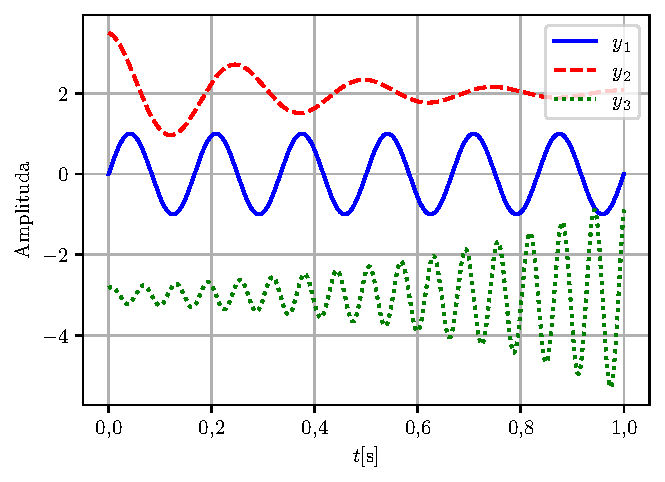
\includegraphics[scale=1]{py_teorija/osc_py.pdf}
    \caption{Primer različitih tipova oscilacija.}
    \label{osc_py}
\end{figure}

\noindent
Na slici \ref{osc_py} su prikazana tri signala oblika
$y_i = O_i + A_i$ sin($2 \pi f_i t - \theta_i$)$e^{-a_it}$. Gde za $y_1$ važi da su $O_1 = 0, A_1 = 1, f_1 = 6, a_1 = 0$, za $y_2$ važi da su $O_2 = 2, A_2 = 1.5, f_2 = 4, a_2 = 3$, i za $y_3$ važi da su $O_3 = -3, A_3 = 0.3, f_3 = 16, a_3 = -2.5$. Ovi signali mogu biti kao što je prethodno napomenuto, napon, struja, dužina, jačina zvuka, itd., zato su vrednosti date kao bezdimenzione radi ilustracije promene oblika signala u odnosu na promenu parametara. Na ovom jednostavnom primeru se može videti da postoji veliki broj načina oscilovanja nekog sistema. Dodatno, na slici \ref{osc_py} su prikazane jednostavnije oscilacije u kojima nema izbijanja ili prenošenja energije sa jednog tela koje osciluje na drugo. Može se vrlo lako zaključiti da naizgled jednostavne, oscilacije mogu veoma lako da postanu komplikovane. Oscilacije su ključne u mnogim područjima fizike, inženjeringa i nauke, te su ključne za razumevanje različitih fenomena u prirodi i tehnologiji.
U ovom radu će fokus biti na osclilacije klatana u fizici.
\cite{fiz}

\subsection{Oscilatori}
Osciatori su uređaju ili sistemi koji generišu oscilacije, odnosno periodične promene u vremenu. Postoji više vrsta oscilatora ali po sprezi se oni mogu podeliti na oscilatore koji su izolovani ili spregnuti, i njihova šema se može videti na slikama \ref{dva_osc} i \ref{spregnuti_osc}, respektivno.

\begin{center}
\begin{minipage}{0.5\textwidth}
\centering
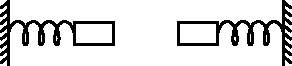
\includegraphics[scale=1.5]{imgs_teorija/dva_odvojena_osc.pdf}
\captionof{figure}{Dva nespregnuta oscilatora.}
\label{dva_osc}
\end{minipage}%\hfill
\begin{minipage}{0.5\textwidth}
\centering
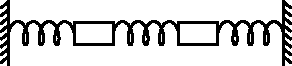
\includegraphics[scale=1.5]{imgs_teorija/spregnuti_osc.pdf} 
\captionof{figure}{Dva spregnuta oscilatora.}  
\label{spregnuti_osc} 
\end{minipage}
\end{center}

\noindent
Na slici \ref{dva_osc}. dva tela mogu da osciluju nezavisno jedno od drugog, dok na slici \ref{spregnuti_osc}. oscilacija jednog tela utiče na oscilacije drugog tela tako što se energija prenosi preko sprege, i ovaj način oscilovanja je komplikovaniji od slučaja kada tela osciluju nezavisno. Postoji više načina sprege oscilatora, na slici \ref{spregnuti_osc}. je ilustrativno prikazan jedan način, ali je suština ista i za druge slučajeve.


\subsection{Klatno}
\subsubsection{Tipovi klatna}
\label{s:mat_klatno}

Klatno predstavlja jedan oscilator koji osciluje oko ravnotežnog položaja. Postoje više tipova klatna: matematičko, fizičko, torziono itd. U ovom radu će fokus biti na fizičkom klatnu. Fizičko klatno predstavlja svako klatno koje ima telo koje je pričvršćeno za neelastičnu šipku (konopac ili štap) koja se može rotirati oko tačke pričvršćivanja. Fizičko klatno se može aproksimirati modelom matematičkog klatna u slučaju da ima veoma dugu neistegljivu šipku zanemarljive mase, i telo koje je zakačeno za kraj šipke velike mase i zanemarljivih dimenzija. Radi izučavanja pojava kod matematičkog klatna potrebno je napraviti model koji zanemaruje sve otporne sile, sem gravitacije. Matematičko klatno se sastoji od tačkaste mase $m$ pričvršćene na idealno neelastičnu šipku dužine $L$ čija masa teži nuli. Ugao između šipke i vertikalne ravni se označava sa $\theta$. Model matematičkog klatna je dat na slici \ref{mat_klatno}.

\begin{figure}[h!]
    \centering
    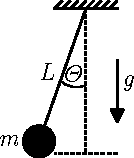
\includegraphics[scale=1.5]{imgs_teorija/mat_klatno.pdf}
    \caption{Model matematičkog klatna.}
    \label{mat_klatno}
\end{figure}



\noindent
Za modelovanje klatna potrebno je izvesti jednačinu kretanja koja se izvodi iz drugog Njutnovog zakona za rotaciju $\tau = I \alpha$, gde je $\tau$ moment gravitacione sile $mg$ oko tačke pričvršćivanja, $I$ moment inercije (za tačkastu masu $m$ i idealno neelastičnu šipku $L$, $I = m L^2$), $\alpha$ je ubrzanje rotacije (drugi izvod ugla $\theta$ po vremenu). Moment sile jednak je proizvodu momenta inercije i ubrzanja rotacije: $mgL$sin$(\theta) = mL^2 \frac{\rm{d}^2 \theta}{\rm{d}t^2}$. Za dalje matematičko sređivanje potrebno je uvesti aproksimaciju $sin(\theta) \approx \theta$ u intervalu ugla od -0.5rad do 0.5rad, što se prevodi u uglove od -30$^\circ$ do 30$^\circ$, i grafici ove dve funkcjie se poklapaju na datom intervalu što se može i videti na slici \ref{theta_approx}. 

\begin{figure}[h!]
    \centering
    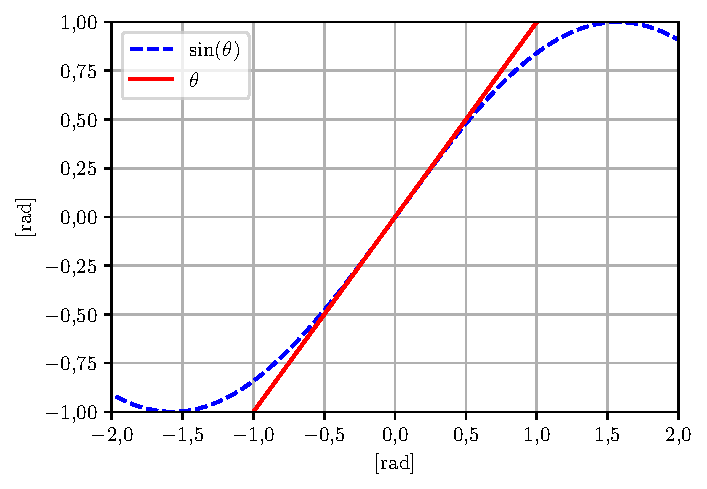
\includegraphics[scale=1]{py_teorija/theta_approx.pdf}
    \caption{Aproksimacija sin($\theta$)$\approx \theta$.}
    \label{theta_approx}
\end{figure}



\noindent
Uzimajući u obzir pomenutu aproksimaciju malog ugla dobija se diferencijalna jednačina kretanja $\frac{\rm{d}^2 \theta}{\rm{d}t^2} + \frac{g}{L}\theta = 0$. Rešenja ove jednačine su sinusne funkcije koje predstavljaju periodične oscilacije sa kružnom učestanošću $\omega$ koja je data formulom (\ref{eq:omega}).

\begin{equation}
\label{eq:omega}
\omega = \sqrt{\frac{g}{L}}
\end{equation}

\noindent
Iz datog izvođenja se može zaključiti da učestanost oscilacija ne zavisi od mase tela koje je zakačeno za neelastičnu šipku, nego samo od dužine šipke i gravitacione sile, što znači da za telo bilo koje mase, ako je dužina neelastične šipke $L$, period oscilacija će biti isti.





\subsubsection{Spregnuta klatna}

U konkretnom eksperimentu su korišćena fizička klatna koja mogu da se aproksimiraju matematičkim klatnom jer im je neelastična šipka male mase,a velike dužine, dok je teg realtivno mali sa velikom masom. Radi lakšeg objašnjavanja principa rada, u daljem tekstu će se koristiti termin matematičko klatno za opisivanje procesa koji se događaju. 

Sistem spregnutih matematičkih klatana predstavlja sistem od dva ili više matematička klatna povezana elastičnom oprugom ili nekim drugim vidom sprege (u ovom radu će se posmatrati samo slučaj za dva spregnuta matematička klatna). Osnovna ideja sprezanja klatna je da se klatna ne ponašaju nezavisno već da utiču jedno na drugo, odnosno, da se dešava transfer energije između njih. Samo kretanje spregnutih klatna je složeno, ali postoje dva tipa kretanja koja se drugačije nazivaju normalni modovi, i oni se javljaju kada su frekvencije oscilovanja klatna veoma bliske, odnosno identične, i tada dolazi do sinhronizacije oscilacija. Primer normalnih modova je dat na slici \ref{spregnuti1} i \ref{spregnuti2}.

\begin{center}
\begin{minipage}{0.5\textwidth}
\centering
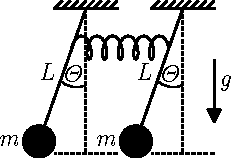
\includegraphics[scale=1.5]{imgs_teorija/spregnuto_klatno_1.pdf}
\captionof{figure}{Normalni mod simetrije.}
\label{spregnuti1}
\end{minipage}%\hfill
\begin{minipage}{0.5\textwidth}
\centering
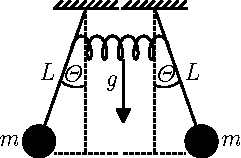
\includegraphics[scale=1.5]{imgs_teorija/spregnuto_klatno_2.pdf} 
\captionof{figure}{Normalni mod antisimetrije.}  
\label{spregnuti2} 
\end{minipage}
\end{center}

\noindent
Kao što se može primetiti, spregnuta matematička klatna mogu da osciluju periodično bez promene u načinu oscilovanja, i to simetrično ili antisimetrično. Svaki drugi način oscilovanja je dosta složeniji jer se dešava transfer energije sa jednog klatna na drugo i to utiče na način oscilovnja klatna. U realnom eksperimentu, veoma je teško podesiti početne pozicije spregnutih klatna da bi ona oscilovala u nekom od pomenutih normalnih modova, već je više verovatno da će se oscilacije biti sa prenosom energije. Ali opet nije nemoguće proceniti kretanje uz pomoć diferencijalnih jednačina. Krećući od jednačine za kinetičku energiju $E_k = \frac{1}{2}mv_1^2 + \frac{1}{2}mv_2^2 = \frac{1}{2}m(l\dot{\theta_1})^2 + \frac{1}{2}m(l\dot{\theta_2})^2$, gde je $v = l \dot{\theta}$, i potencijalu energiju $E_p = -mgl$cos($\theta_1$) $-mgl$cos($\theta_2$)$+\frac{1}{2}k$($l$sin($\theta_2$)$-l$sin($\theta_1$))$^2$, gde je referentna tačka nultog potencijala mesto vešanja neelastične šipke, dok je $k$ koeficijent sprege opruge, a razlika sinusa u trećem članu u jednačini predstavlja ukupno istezanje sistema. Korišćenjem Lagranžijana, $L = E_k - E_p$, aproksimaciju: sin($\theta$)$\approx \theta$, za male uglove $\theta$ objašnjenu u delu \ref{s:mat_klatno} i prikazanu na slici \ref{theta_approx}., kao i aproksimaciju: cos($\theta$)$\approx 1 - \frac{\theta^2}{2}$, što je prikazano na slici \ref{cos_approx}. dobija se: 

\begin{equation}
L = \frac{1}{2}ml^2\dot{\theta_1^2} + \frac{1}{2}ml^2\dot{\theta_2^2} - \frac{1}{2}mgl\theta_1^2 - \frac{1}{2}mgl\theta_2^2 - \frac{1}{2}kl^2(\theta_2 - \theta_1)^2 + 2mgl
\label{eq:Lagranzijan}
\end{equation}



\noindent
Kako bi se došlo do izraza za $\theta(t)$ potrebno je rešiti Ojlerove diferencijalne jednačine: $\frac{d}{dt} \left( \frac{\partial L}{\partial \dot{\theta_1}} \right) - \frac{\partial L}{\partial \theta_1} = 0$, i $\frac{d}{dt} \left( \frac{\partial L}{\partial \dot{\theta_2}} \right) - \frac{\partial L}{\partial \theta_2} = 0$. Korišćenjem ovih izraza i jednačine (\ref{eq:Lagranzijan}), lako se dolazi do diferencijalnih jednačina kretanja za oba klatna: 


\begin{equation}
\ddot{\theta_1} + \frac{g}{l} \theta_1 - \frac{k}{m}(\theta_2 - \theta_1) = 0
\label{eq:diff1}
\end{equation}

\begin{equation}
\ddot{\theta_2} + \frac{g}{l} \theta_2 + \frac{k}{m}(\theta_2 - \theta_1) = 0
\label{eq:diff2}
\end{equation}


\begin{figure}[h!]
    \centering
    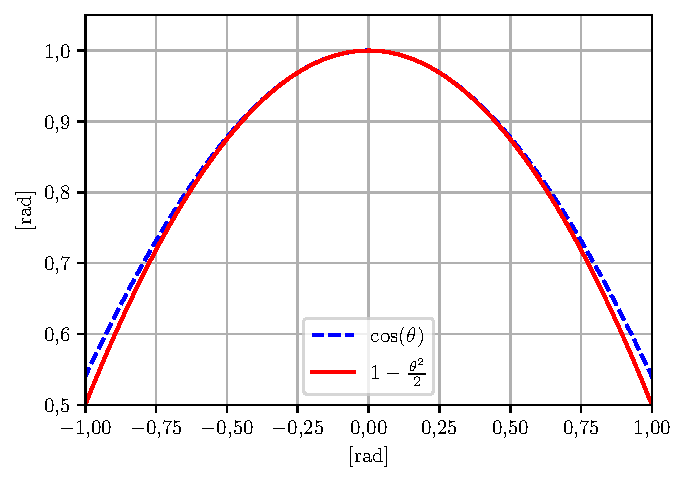
\includegraphics[scale=1]{py_teorija/cos_approx.pdf}
    \caption{Aproksimacija cos($\theta$)$\approx 1-\frac{\theta^2}{2}$.}
    \label{cos_approx}
\end{figure}

Rešavanjem diferencijalnih jednačina kretanja (\ref{eq:diff1}) i (\ref{eq:diff2}), uz korišćenje matričnog zapisa diferencijalne jednačine, lako se dolazi do rešenja, odnosno jednačine kretanja za oba klatna i one su date kao:

\begin{equation}
\theta_1(t) = C_1cos(\omega_1t) + C_2cos(\omega_2t)
\end{equation}

\begin{equation}
\theta_2(t) = C_1cos(\omega_1t) - C_2cos(\omega_2t)
\end{equation}

\noindent
gde su $C_1$ i $C_2$ koeficijenti koji zavise od početnih uslova sistema, dok $\omega_1$ i $\omega_2$ predstavljaju sopstvene kružne učestanosti sistema prikazanog na slikama \ref{spregnuti1}. i \ref{spregnuti2}., i lako se pokazuje iz jednačine (\ref{eq:Lagranzijan}) da važi: $\omega_1 = \sqrt{\frac{g}{l}}$ i $\omega_2 = \sqrt{\frac{g}{l} + \frac{2k}{m}}$.

Ove jednačine su veoma bitne jer je moguće simulirati eksperiment i videti koji su očekivani rezultati merenja. Za potrebe simulacije je napisana Python skripta koja uzima u obzir i gubitke energije oscilacija usled trenja o tačku vešanja kao i otpora vazduha. Naravno, u realnom eksperimentu će biti dodatni mali otpori koji se ne mogu predvideti i tačno sračunati simulacijom. Zbog toga su za parametre simulacije su uzete pokazne vrednosti, jer je akcenat dat na pokazivanje prirode kretanja. Rezultati simulacije kretanja spregnutog matematičkog klatna $\theta_1(t)$ i $\theta_2(t)$ su prikazani na slici \ref{sim_kretanja}.


\begin{figure}[h!]
    \centering
    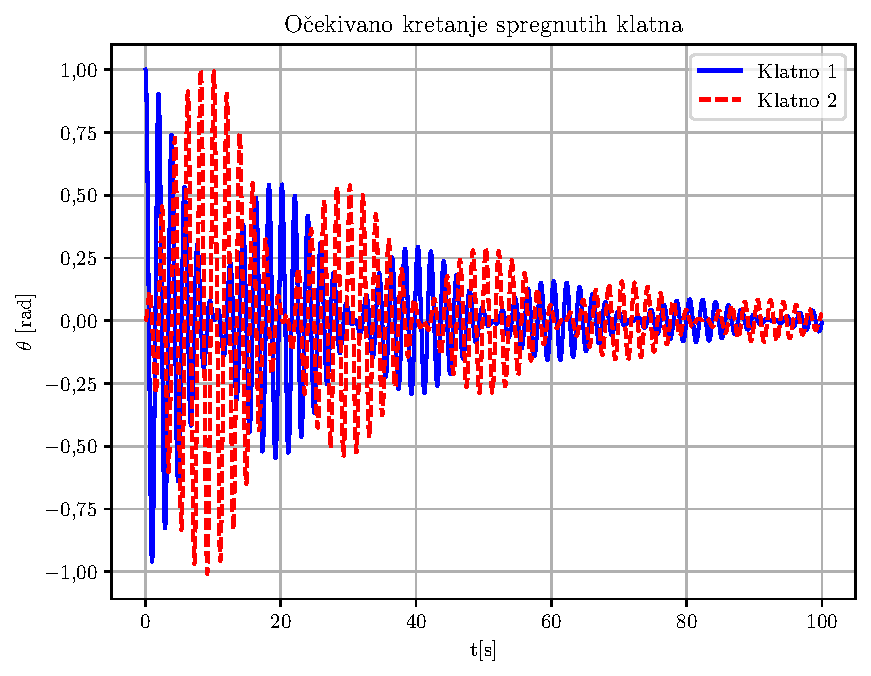
\includegraphics[scale=0.9]{py_teorija/spregnuto_mat.pdf}
    \caption{Očekivano kretanje spregnutih matematičkih klatna.}
    \label{sim_kretanja}
\end{figure}


\begin{figure}[h!]
    \centering
    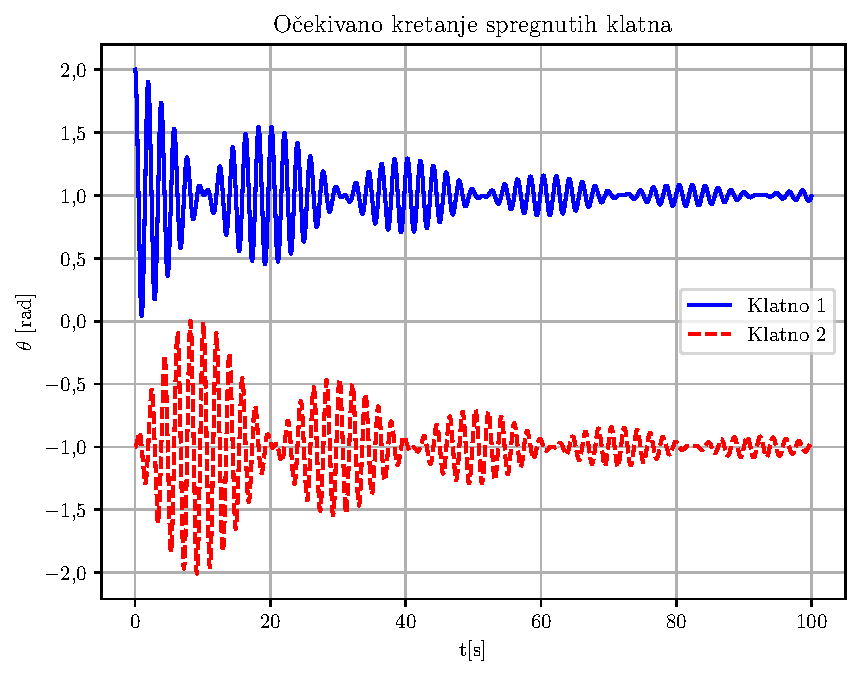
\includegraphics[scale=0.9]{py_teorija/spregnuto_mat2.pdf}
    \caption{Očekivano kretanje spregnutih matematičkih klatna (odvojeno).}
    \label{sim_kretanja2}
\end{figure}

\noindent
Na slici \ref{sim_kretanja} su prikazane funkcije kretanja $\theta_1(t)$ i $\theta_2(t)$ preklopljene jedna preko druge, dok su radi lakšeg razumevanja one odvojene na slici \ref{sim_kretanja2}.

\noindent
Na slici \ref{sim_kretanja2}. se jasnije može videti da amplitude oscilacija oba klatna variraju i da dolazi i do zaustavljanja oscilacija jednog klatna kada je drugo klatno u lokalnom maksimumu. Ovo je primer kada je jedno klatno izvedeno iz ravnotežnog položaja i pušteno da osciluje dok je drugo ostalo u ravnotežni položaj. Zato se ovo rešenje može smatrati opštim rešenjem kretanja, dok, da bi se dobila dva specifična načina kretanja, odnosno normalni modovi, potrebno je da početni uslovi budu takvi da su oba klatna pomerena za početni ugao $\theta_0$ od ravnotežnog položaja, ili da je jedno klatno pomereno za $+\theta_0$, a drugo za $-\theta_0$, i time se dobijaju normalni mod simetrije prikazan na slici \ref{spregnuti1}., i normalni mod antisimetrije prikazan na slici \ref{spregnuti2}., respektivno. Rezultati simulacije za normalne modove su prikazane na slikama \ref{nmod1}. i \ref{nmod2}.

\begin{figure}[h!]
    \centering
    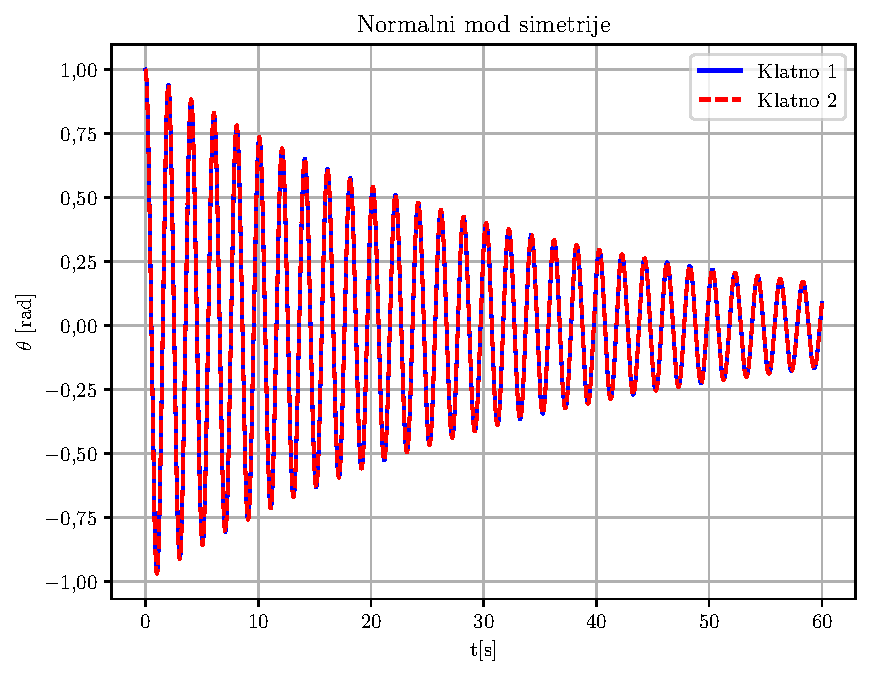
\includegraphics[scale=0.9]{py_teorija/nmod_simetrija.pdf}
    \caption{Simulacija kretanja usled normalnog moda simetrije.}
    \label{nmod1}
\end{figure}

\break

\begin{figure}[h!]
    \centering
    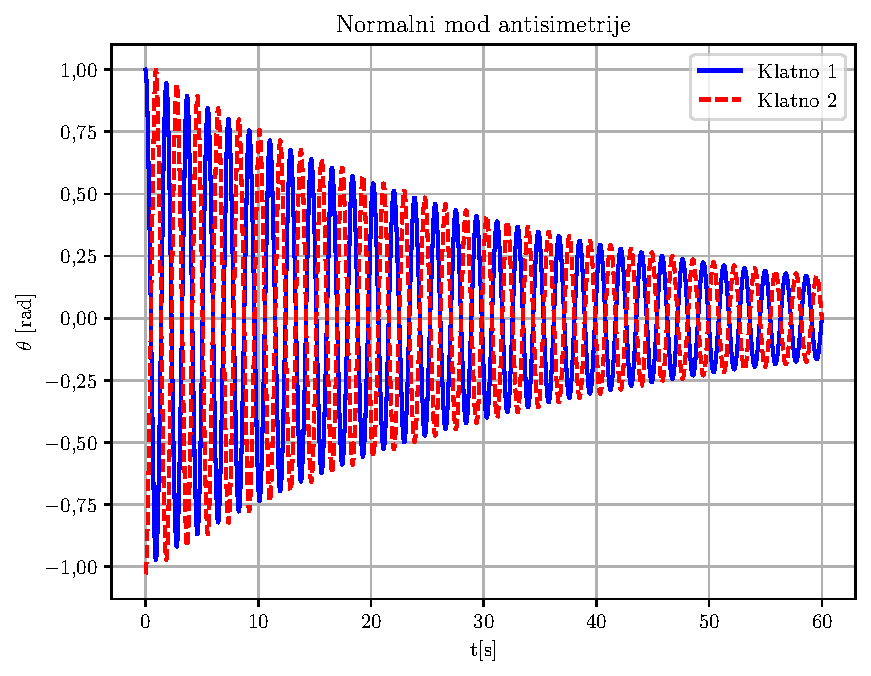
\includegraphics[scale=0.9]{py_teorija/nmod_asimetrija.pdf}
    \caption{Simulacija kretanja usled normalnog moda antisimetrije.}
    \label{nmod2}
\end{figure}


\noindent
Usled normalnog moda simetrije, kretanje je identično i važi relacija $\theta_1(t) = \theta_2(t)$, što je prikazano na slici \ref{nmod1}. Usled normalnog moda antisimetrije, kretanje je suprotno i važi relacija $\theta_1(t) = -\theta_2(t)$, što je prikazano na slici \ref{nmod2}. 
\cite{mit}
\cite{dos}



\subsection{Rotacioni enkoder}
Uloga enkodera je da obezbeđuje informaciju o trenutnom položaju, odnosno smeru okretanja osovine. Enkoder je sačinjen iz diska priključenog za osovinu rotora, i na sebi ima proreze kroz koje može da prođe svetlost. S jedne strane je optički uređaj koji emituje svetlosne zrake dok je s druge strane optički uređaj koji ih prima. Ako se taj svetlosni signal prevede u električni, imaće oblik povorke pravougaonih impulsa. Dodatno, ako enkoder ima opciju da daje informaciju o smeru, jedna od implementacija je da se ispod postojećih proreza nalazi još jedan set proreza koji je celokupno pomeren u jednu stranu u odnosu na proreze iznad. 
Na taj način se dobijaju dva signala, signal \navod{u fazi} i signal \navod{u kvadraturi}, od kojih je jedan fazno pomeren u vremenu. U odnosu na to koji od signala prednjači, može se jednoznačno imati informacija o smeru kretanja. Na slici \ref{enc} je ilustrativno pokazan princip rada enkodera.


\begin{figure}[h!]
    \centering
    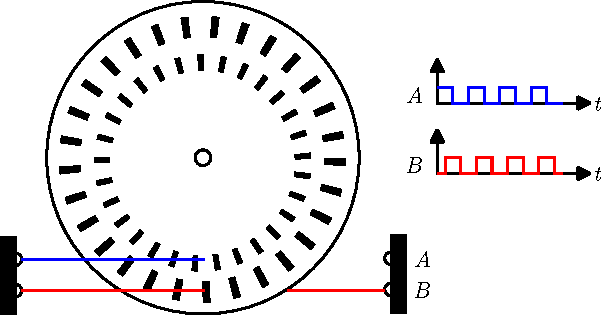
\includegraphics[scale=1]{fig/enc.pdf}
    \caption{Enkoder.}
    \label{enc}
\end{figure}


Konačno, ako se zna broj proreza na enkoderu može se odrediti i ugaona brzina motora $\upomega_{\rm m}$ uz minimalnu grešku koja se svodi na preciznost merenja. U ovom radu je korišćen motor stalne struje sa ugrađenim enkoderom koji radi na ovom principu. Radi jednostavnosti, u ovom radu razmatra se upravljanje brzine motora bez promene smera okretanja, na osnovu čega se koristi samo jedan signal.
\cite{encArduino}


\subsection{Akvizicija podataka} 
\label{sec:Akvzicija} \label{s:Akvizicija}

Nakon teorijskih proračuna gde se uzimaju u obzir idealni uslovi, potrebno je isprojektovati eksperimentalnu postavku i izmeriti dobijene rezultate. Merenje se može odraditi na više načina, ali najpreciznije i najbrže je uz korišćenje računara. U konkretnom slučaju potrebno je meriti kretanje spregnutih matematičkih klatana uz pomoć računara. Najjednostavniji način je da se iskoristi enkoder na mestu vešanja klatna, arduino razvojna ploča, i računar. Skica sistema se može videti na slici \ref{akvizicija}.


\begin{figure}[h!]
    \centering
    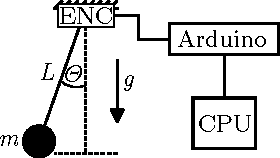
\includegraphics[scale=1.5]{imgs_teorija/akvizicija.pdf}
    \caption{Model sistema za akviziciju signala o položaju klatna.}
    \label{akvizicija}
\end{figure}

\noindent
Osnovni princip akvizicije signala je postavljanje adekvatnog senzora (rotacioni enkoder), zatim pojačavači, filtri, multiplekser, prati-pamti kolo, i AD konvertor (Arduino), i na kraju CPU, odnosno računar.
Enkoder se relativno lako povezuje na Arduino preko ulaznih pinova, a i Arduino se sa računarom lako povezuje USB portom. USB je serijski port, a Arduino prima podatke sa enkodera paralelno. Arduino ima u sebi i univerzalni asinhroni primopredajnik (UART) koji je zadužen za konverziju paralelnih podataka u serijske i time omogućava vezu sa računarom.
\cite{ems} \\

Cilj ovog poglavlja je da detaljnije teorijski opiše delove sistema, kao i teorijska očekivanja ponašanja sistema koji je potrebno isprojektovati.



\newpage

\section{Karakteristike korišćenih komponenti sistema}
\label{sec:Karakteristike}

U ovom poglavlju, akcenat je dat na opisivanje komponenti sistema korišćenih za dobijena merenja.

\subsection{Karakteristike klatna}

U teoriji, matematičko klatno predstavlja sistem od neelastične šipke zanemarljive mase koja teži nuli, i tačkaste mase okačene na kraj te šipke. U realnom eksperimentu šipka ima svoju masu, dok telo okačeno na kraj šipke nije tačkasto nego ima konačne dimenzije. Realno klatno se može aproksimirati teorijskim matematičkim klatnom ako je masa šipke zanemarljiva u odnosu na masu tela okačenog na njen kraj, i ako su dimenzije tela okačenog na šipku zanemarljive u odnosu na dimenzije šipke. Dalja merenja su rađena pod aproksimacijom da se radi sa matematičkim klatnima umesto fizičkim. Finalna postavka relnog klatna koje je korišćeno za merenja je prikazano na slici \ref{eksperiment1}. 


\begin{figure}[h!]
    \centering
    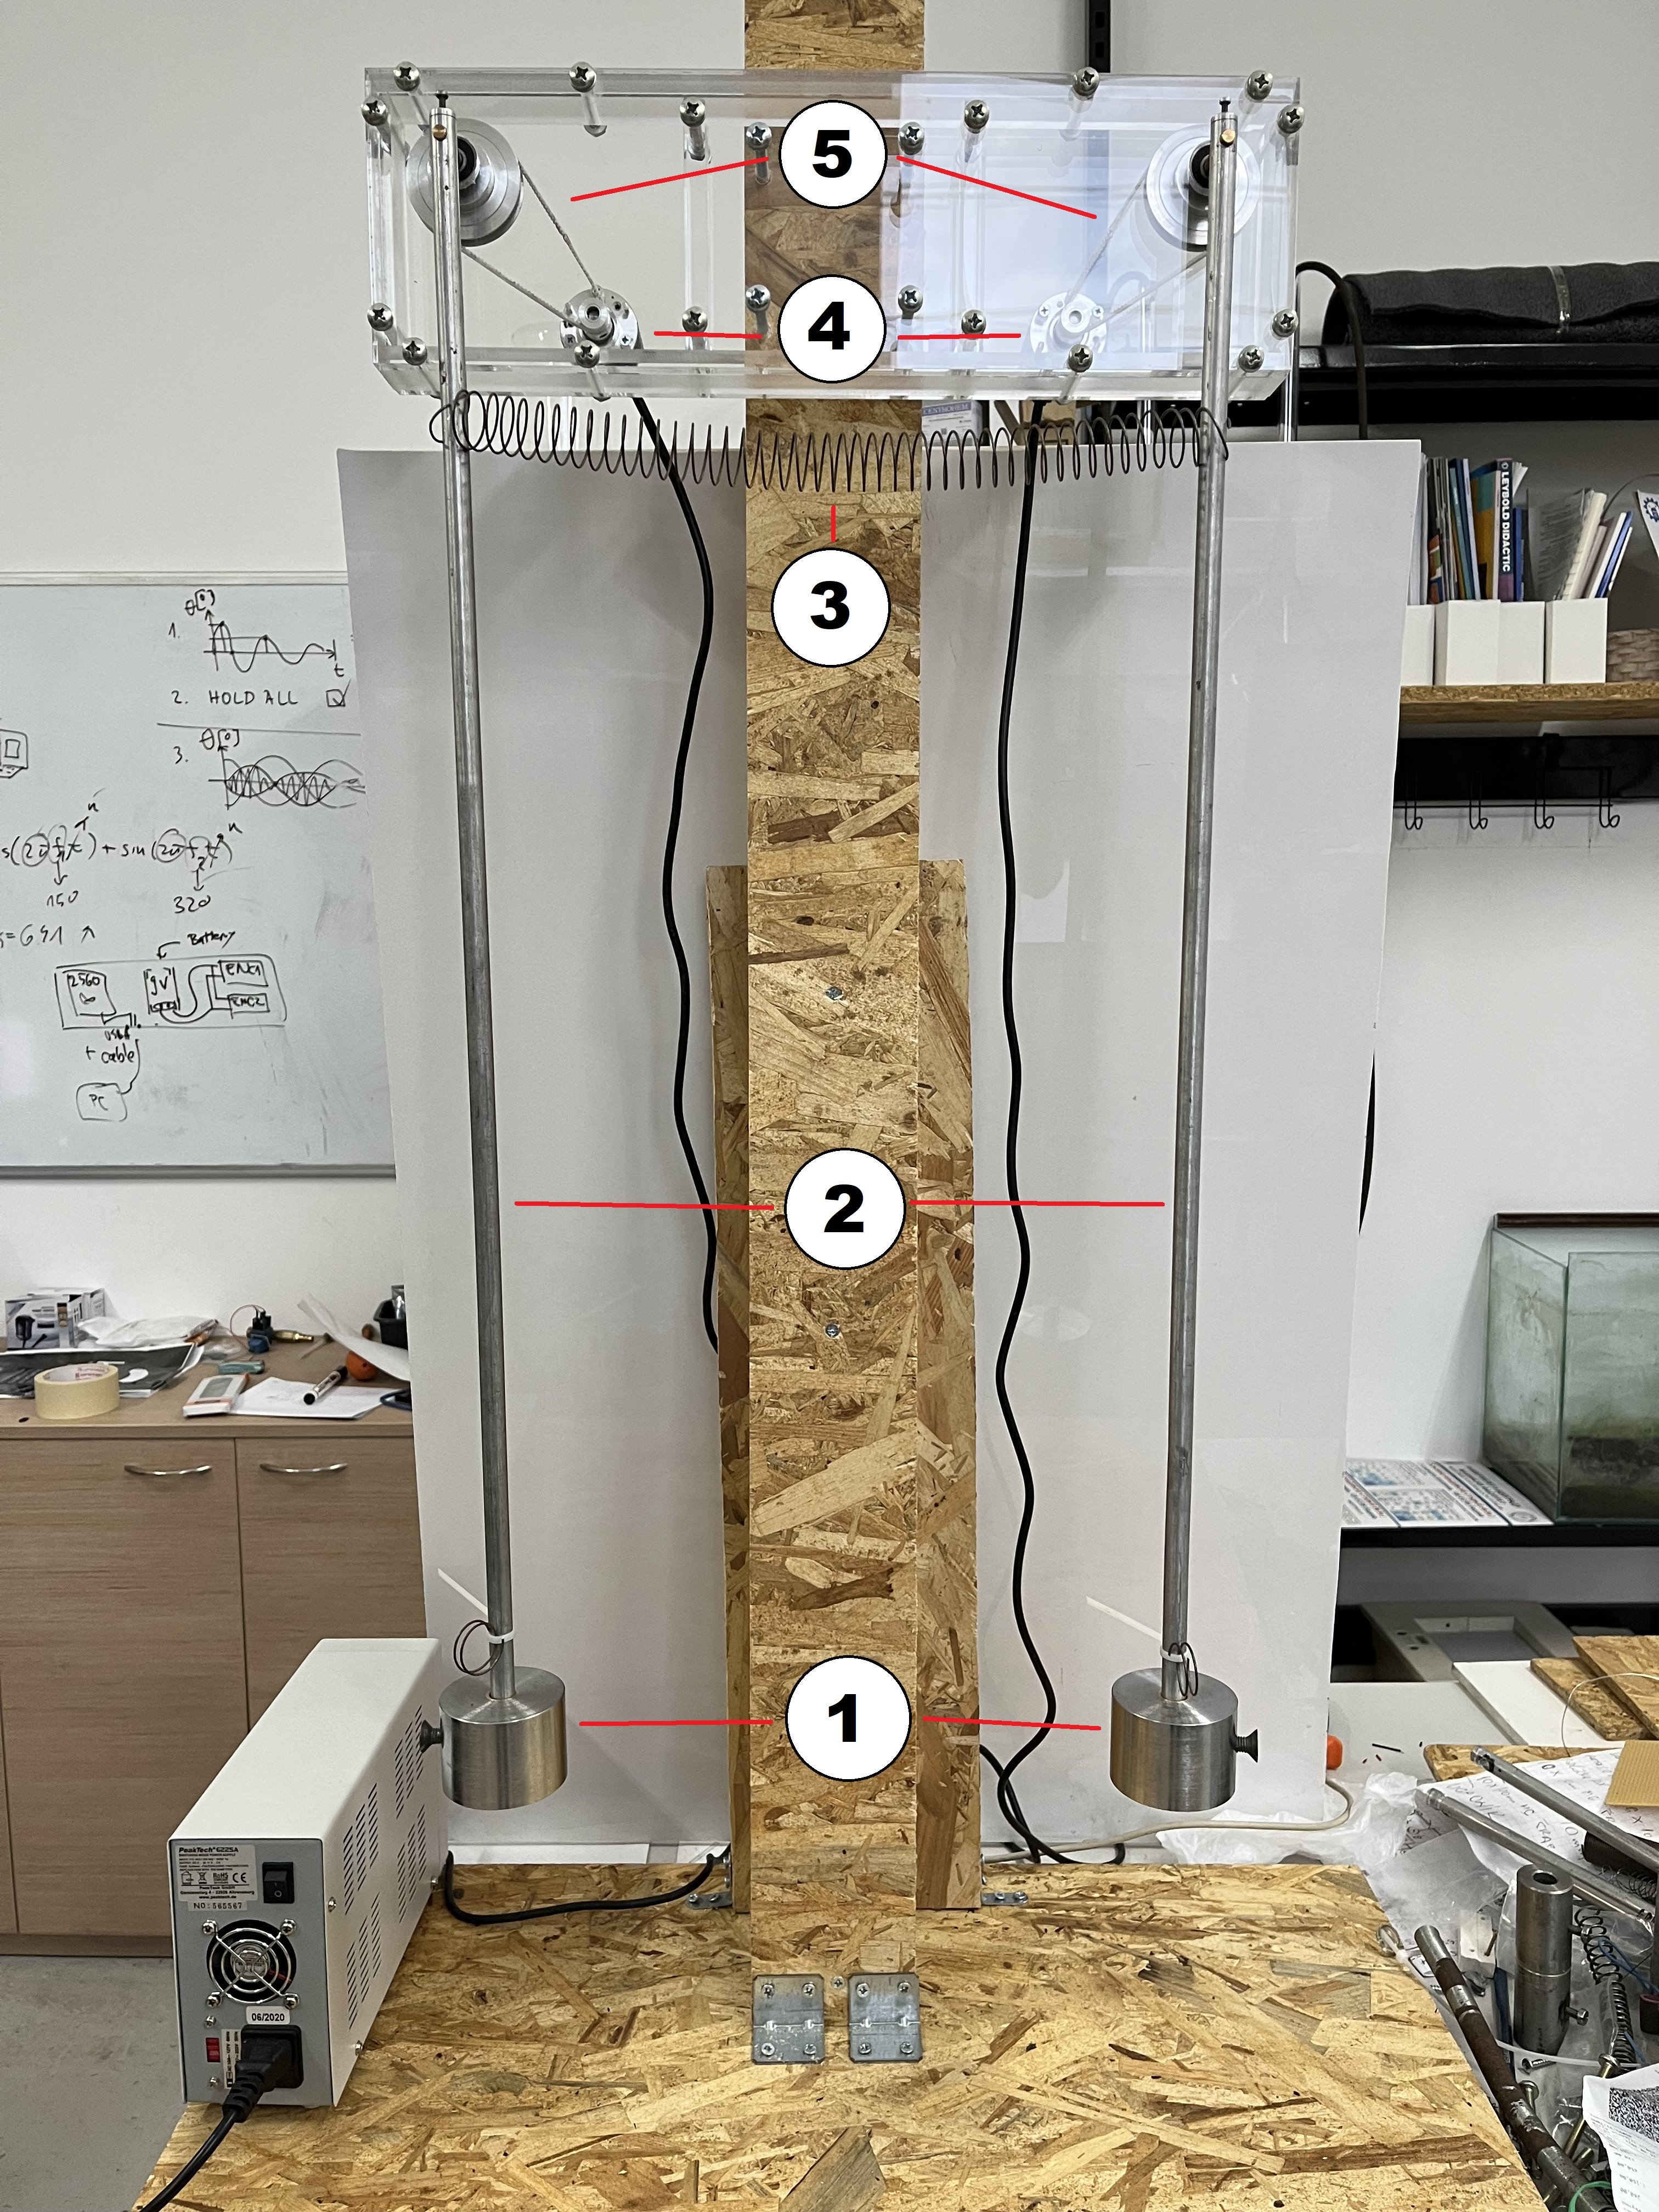
\includegraphics[angle=0,width=0.55\textwidth]{real/klatno2.jpeg}
    \caption{Eksperimentalna postavka spregnutih klatana.}
    \label{eksperiment1}
\end{figure}

\noindent
Na slici \ref{eksperiment1}. su brojevima označeni ključni delovi sistema. 1 - tegovi, 2 - neistegljive šipke, 3 - elastična opruga (sprega), 4 - enkoderi i 5 - sistem za povećanje prenosnog odnosa koji je detaljnije prikazan na slici \ref{prenos}.


\begin{figure}[h!]
    \centering
    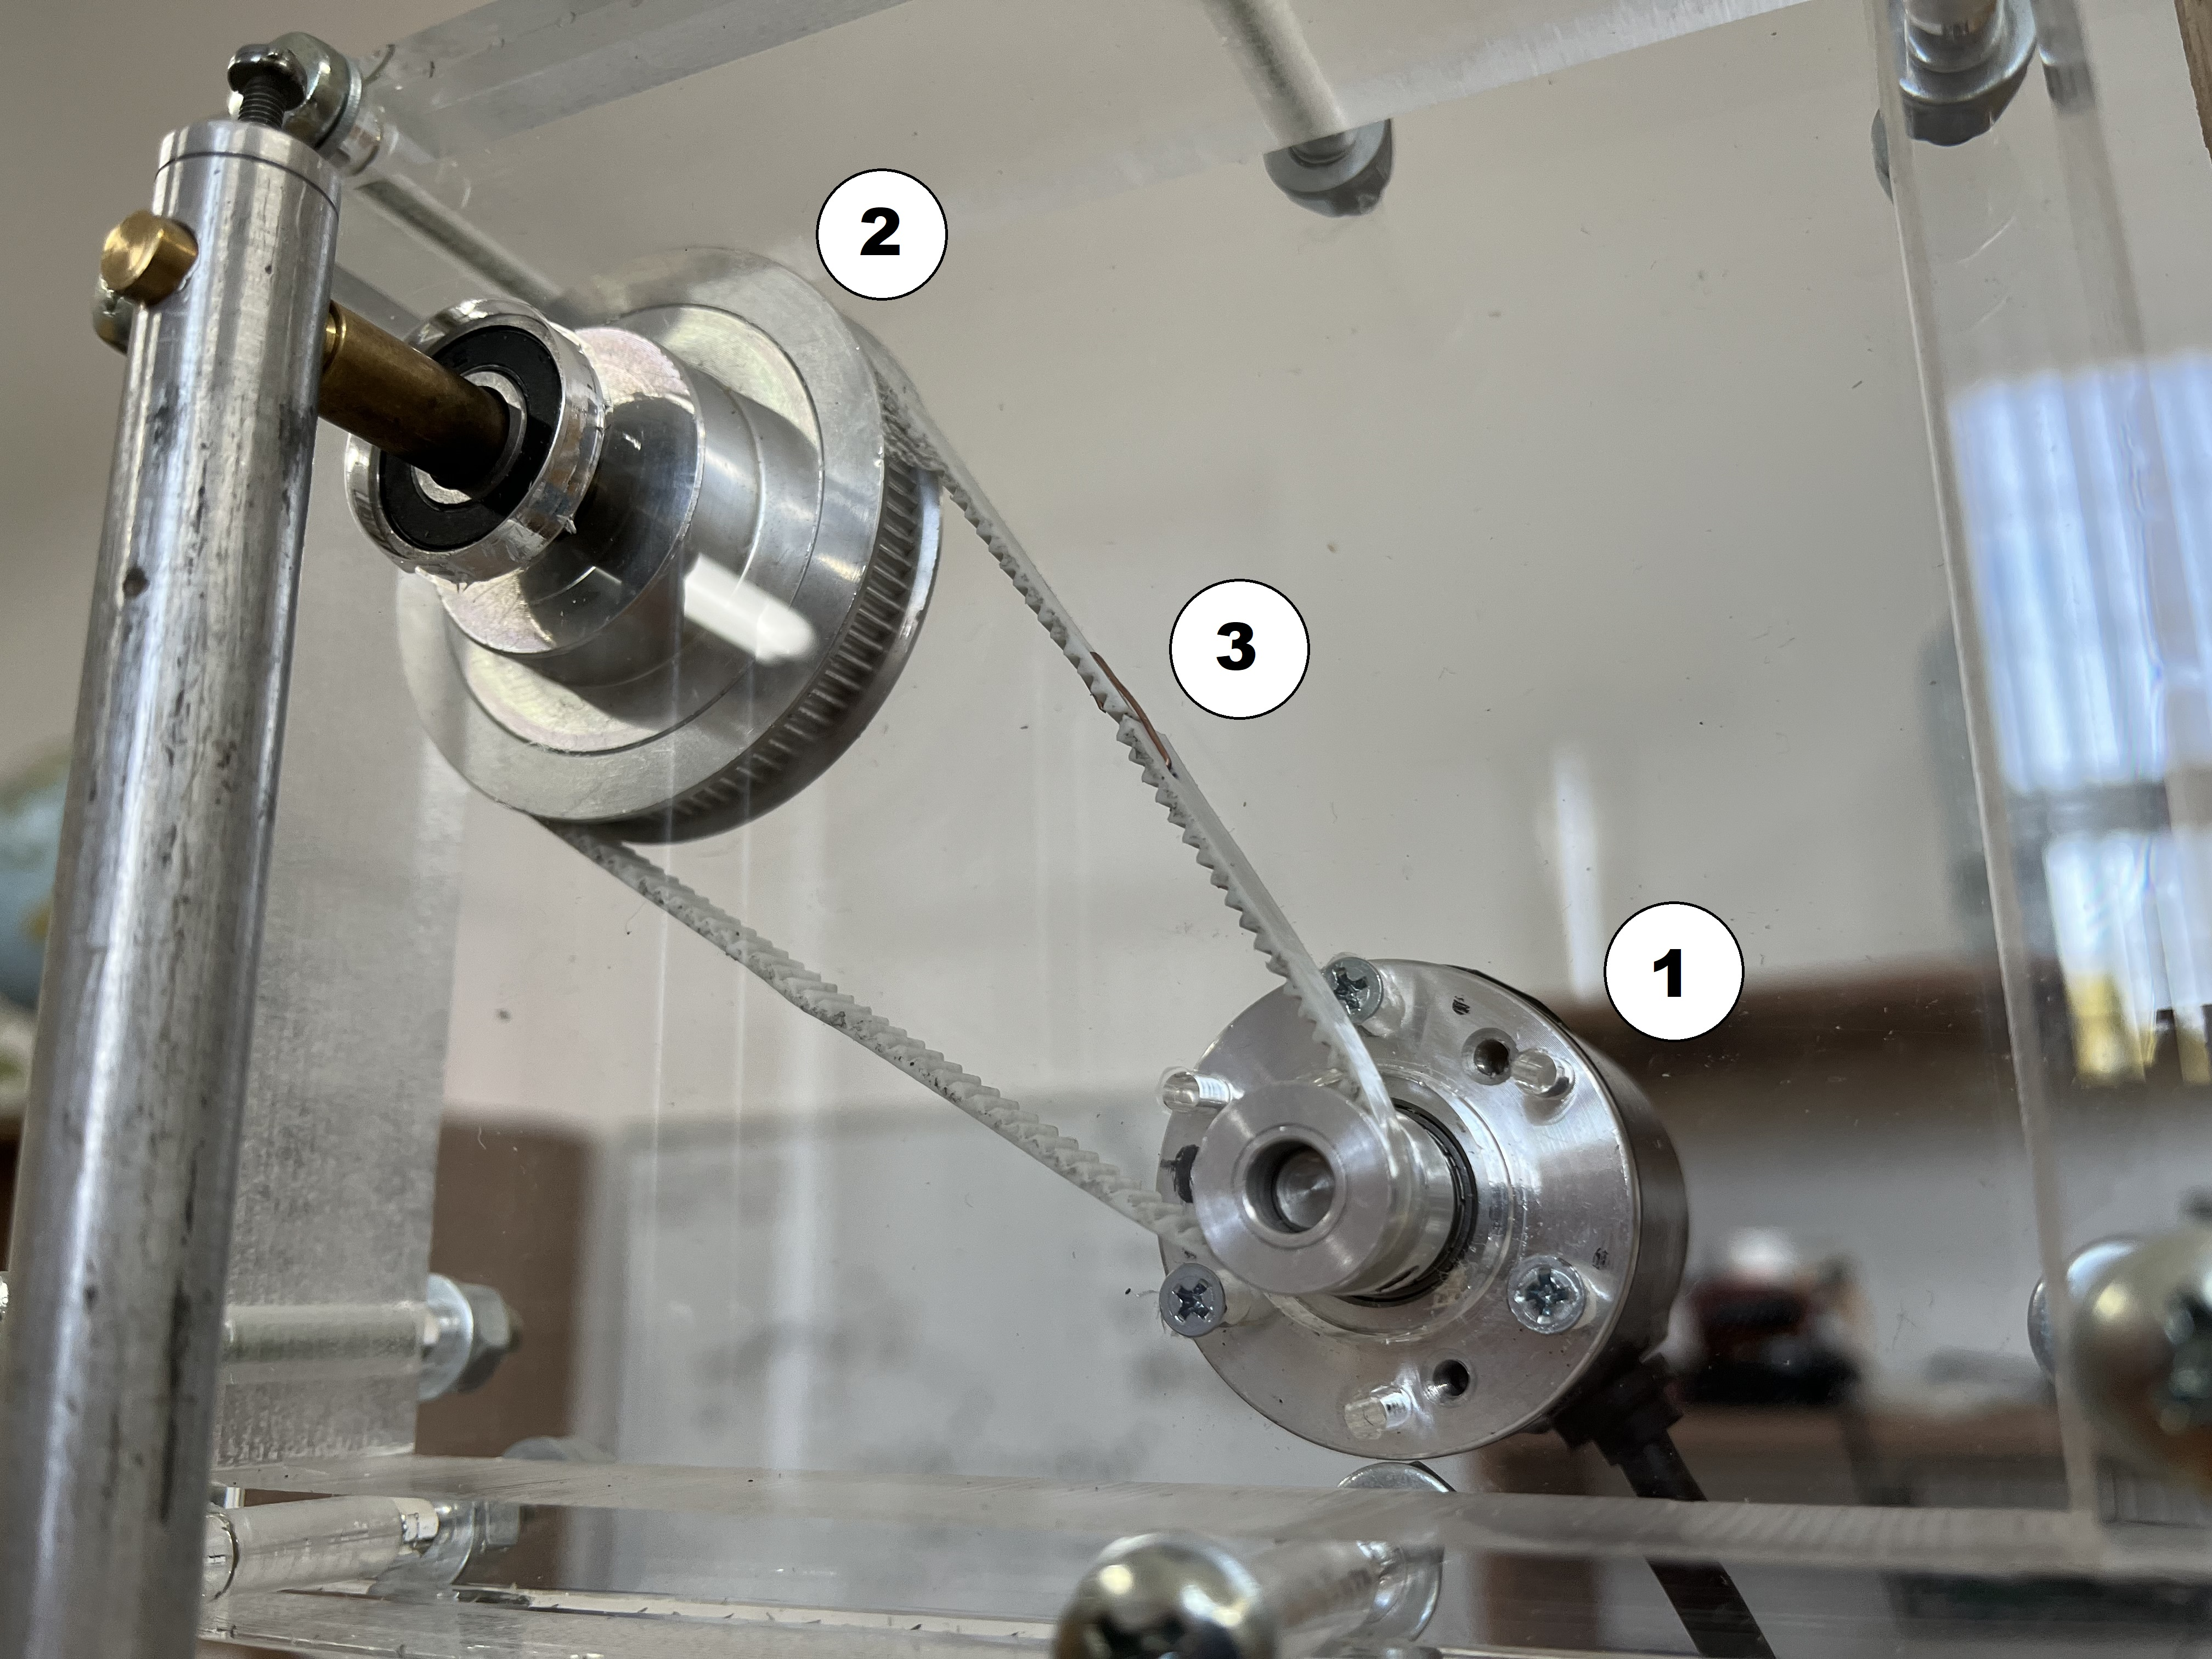
\includegraphics[angle=0,width=0.7\textwidth]{real/prenos2.jpeg}
    \caption{Sistem za povećanje prenosnog odnosa.}
    \label{prenos}
\end{figure}

\noindent
Brojem 1 je označen enkoder sa dodatkom za osovinu sa 16 zubaca. Brojem 2 je označen dodatak sa 80 zubaca na osovini za koju je zakačeno klatno.  Brojem 3 je označen neistegljivi zubčasti kaiš koji omogućava prenos. Ovakvom modifikacijom je omogućeno povećane prenosnog odnosa 5 puta, i samim tim povećanjem i preciznosti.


\subsection{Karakteristike rotacionog enkodera}

Model rotacionog enkodera koji je korišćen je HN3806-AB-1000N. HN3806 Fotoelektrični inkrementalni dvofazni (AB) NPN rotacioni enkoder [5V-24V] koji se koristi za detekciju i merenje položaja ili brzine rotacije objekta prema položaju ugla kretanja. Rotacioni enkoder, poznat i kao osovinski enkoder, elektromehanički je pretvarač koji konvertuje položaj ugla ili kretanje, u električni signal (digitalni ili analogni signal). Pomenuti pretvarač koristi optičku senzorsku tehnologiju koja pruža najtačnije rezultate sa visokom rezolucijom. Pomenuti inkrementalni enkoder konvertuje položaj ugla svog rotora u povorku pravougaonih impulsa (AB dvofazni) koristeći rotirajući rešetkasti disk i optokapler.
Enkoder HN3806 može se koristiti za detekciju i merenje ugla, brzine, dužine i ubrzanja željenih objekata, što je korisno za pametno upravljanje bilo kojim pomeranjem i fiksnom dužinom u CNC mašinama, povratnoj informaciji motora i bilo kojim sistemima zatvorenih petlji. Pomenuti enkoder je baziran na metalnoj konstrukciji, pa je robusan i čvrst, što je idealno za zahtevne industrijske uslove kao što su bušenje na naftnim bušotinama, industrijska kontrola mašina, automatizacija poljoprivrede, kontrola procesa na kanapu, robotika, liftovi, građevinska oprema, kranovi, i tako dalje. Korišćeni enkoder je prikazan na slici \ref{enc2}. 


\begin{figure}[h!]
    \centering
    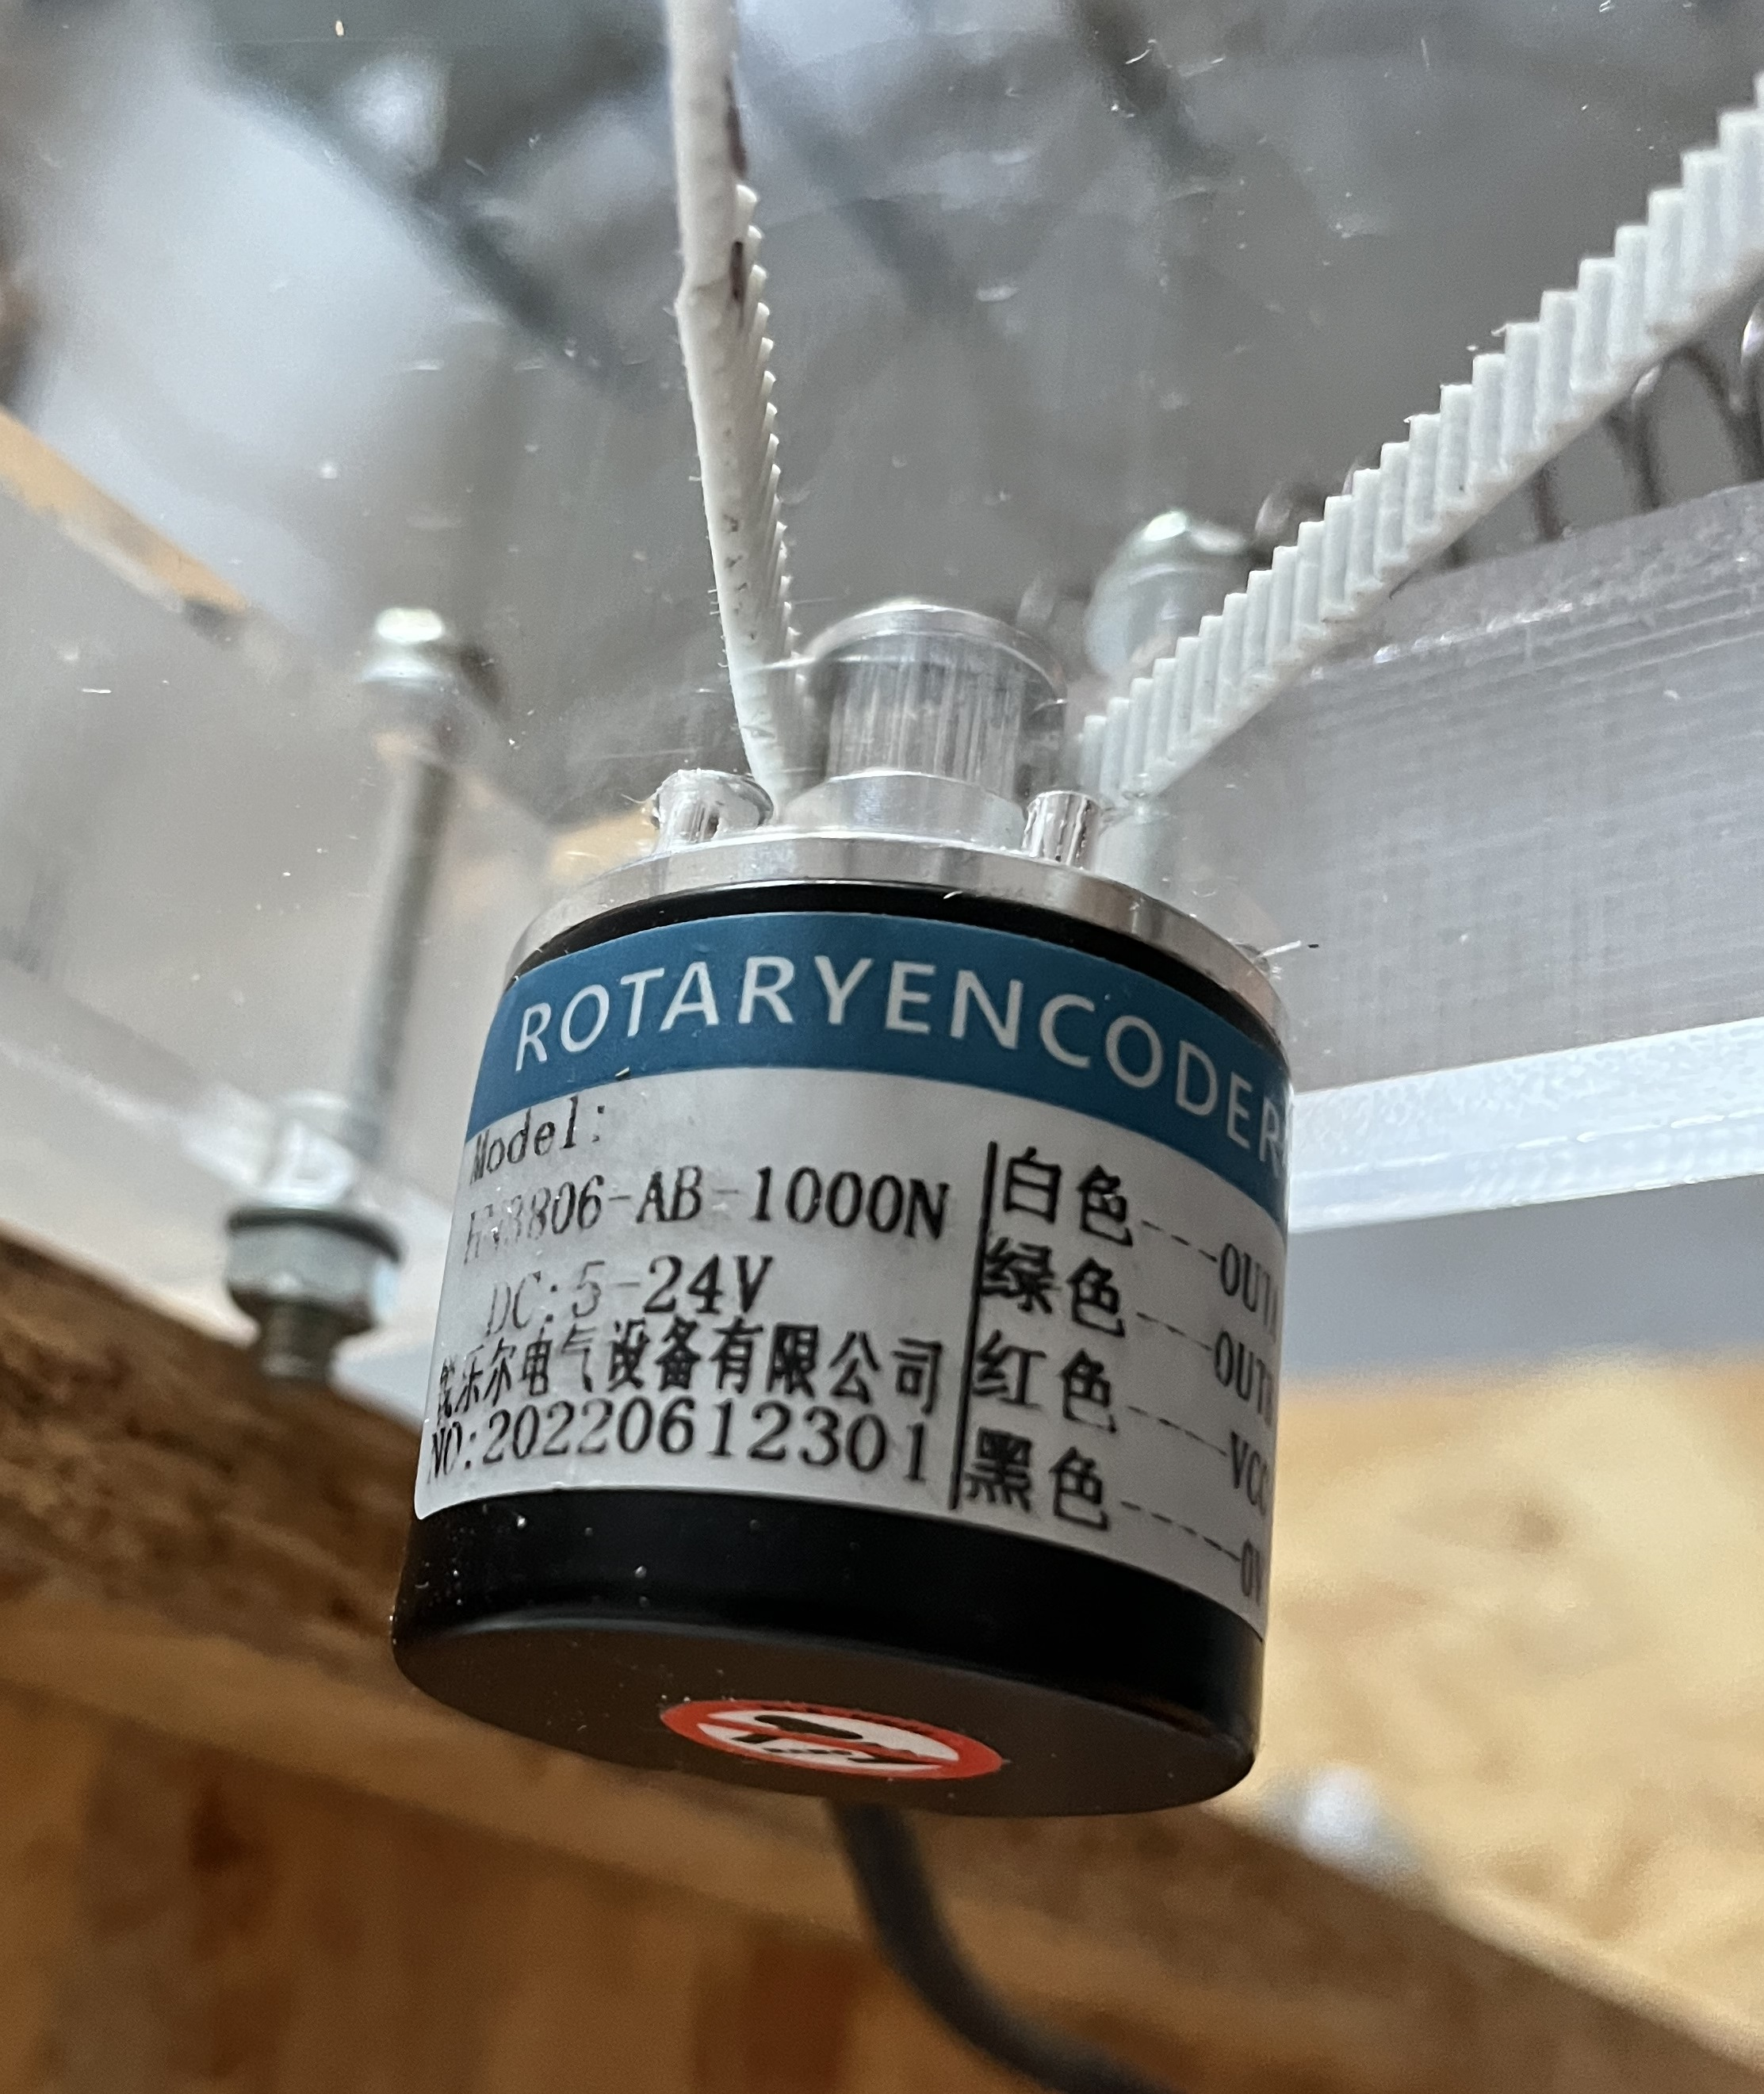
\includegraphics[angle=0,width=0.5\textwidth]{imgs_real/enc2.jpeg}
    \caption{HN3806-AB-1000N rotacioni enkoder.}
    \label{enc2}
\end{figure}


\noindent
Pomenuti enkoder ima 1000 impulsa na 360$^{\circ}$, odnosno preciznost od 0.36$^{\circ}$, što može delovati kao dobra preciznost ali nije dovoljna jer je teško detektovati da li taj impuls potiče od šuma ili pomeraja kada su u pitanju male oscilacije. Kao što se može zaključiti iz specifikacije enkodera, i pored svoje preciznosti, nije namenjen za fina merenja pa je potrebno napraviti odgovarajući prenos uz pomoć zupčanika kako bi se još povećala preciznost pri malim promenama ugla. Dodatno, priključci koje ima ovaj rotacioni enkoder su Pozitivan kraj napajanja (crvena žica), masa (crna žica), signal A (zelena žica) i signal B (bela žica).

\subsection{Eksterno napajanje}

Eksterna napajanja se koriste kako bi sistemima omogućila potrebnu snagu za rad. U datoj postavci jedina komponenta koja daje napajanje je Arduino koji daje 3.3V ili 5V jednosmernog napona koji može potencijalno da osciluje oko te vrednosti. Dok je za napajanje enkodera potreban minimalan napon od 5V. Može doći do problema jer to nije dovoljan napon za ispravan rad enkodera. Iako su na papiru potrebne specifikacije napajanja zadovoljene, to ne mora da znači da će biti omogućen ispravan rad usled grešaka u proizvodnji enkodera. Siguran način da se obezbedi ispravan rad je da se ne radi sa naponima napajanja koji su blizu granica 5V ili 24V, već da se koriste naponi napajanja unutar granica, bliži sredini opsega. Zato je iskorišćeno eksterno podesivo napajanje uz pomoć kojeg su dobijeni legitimni rezultati. Konkretno, korišćeno je napajanje PeakTech 6225A koje je prikazano na slici \ref{napajanje}.


\begin{figure}[h!]
    \centering
    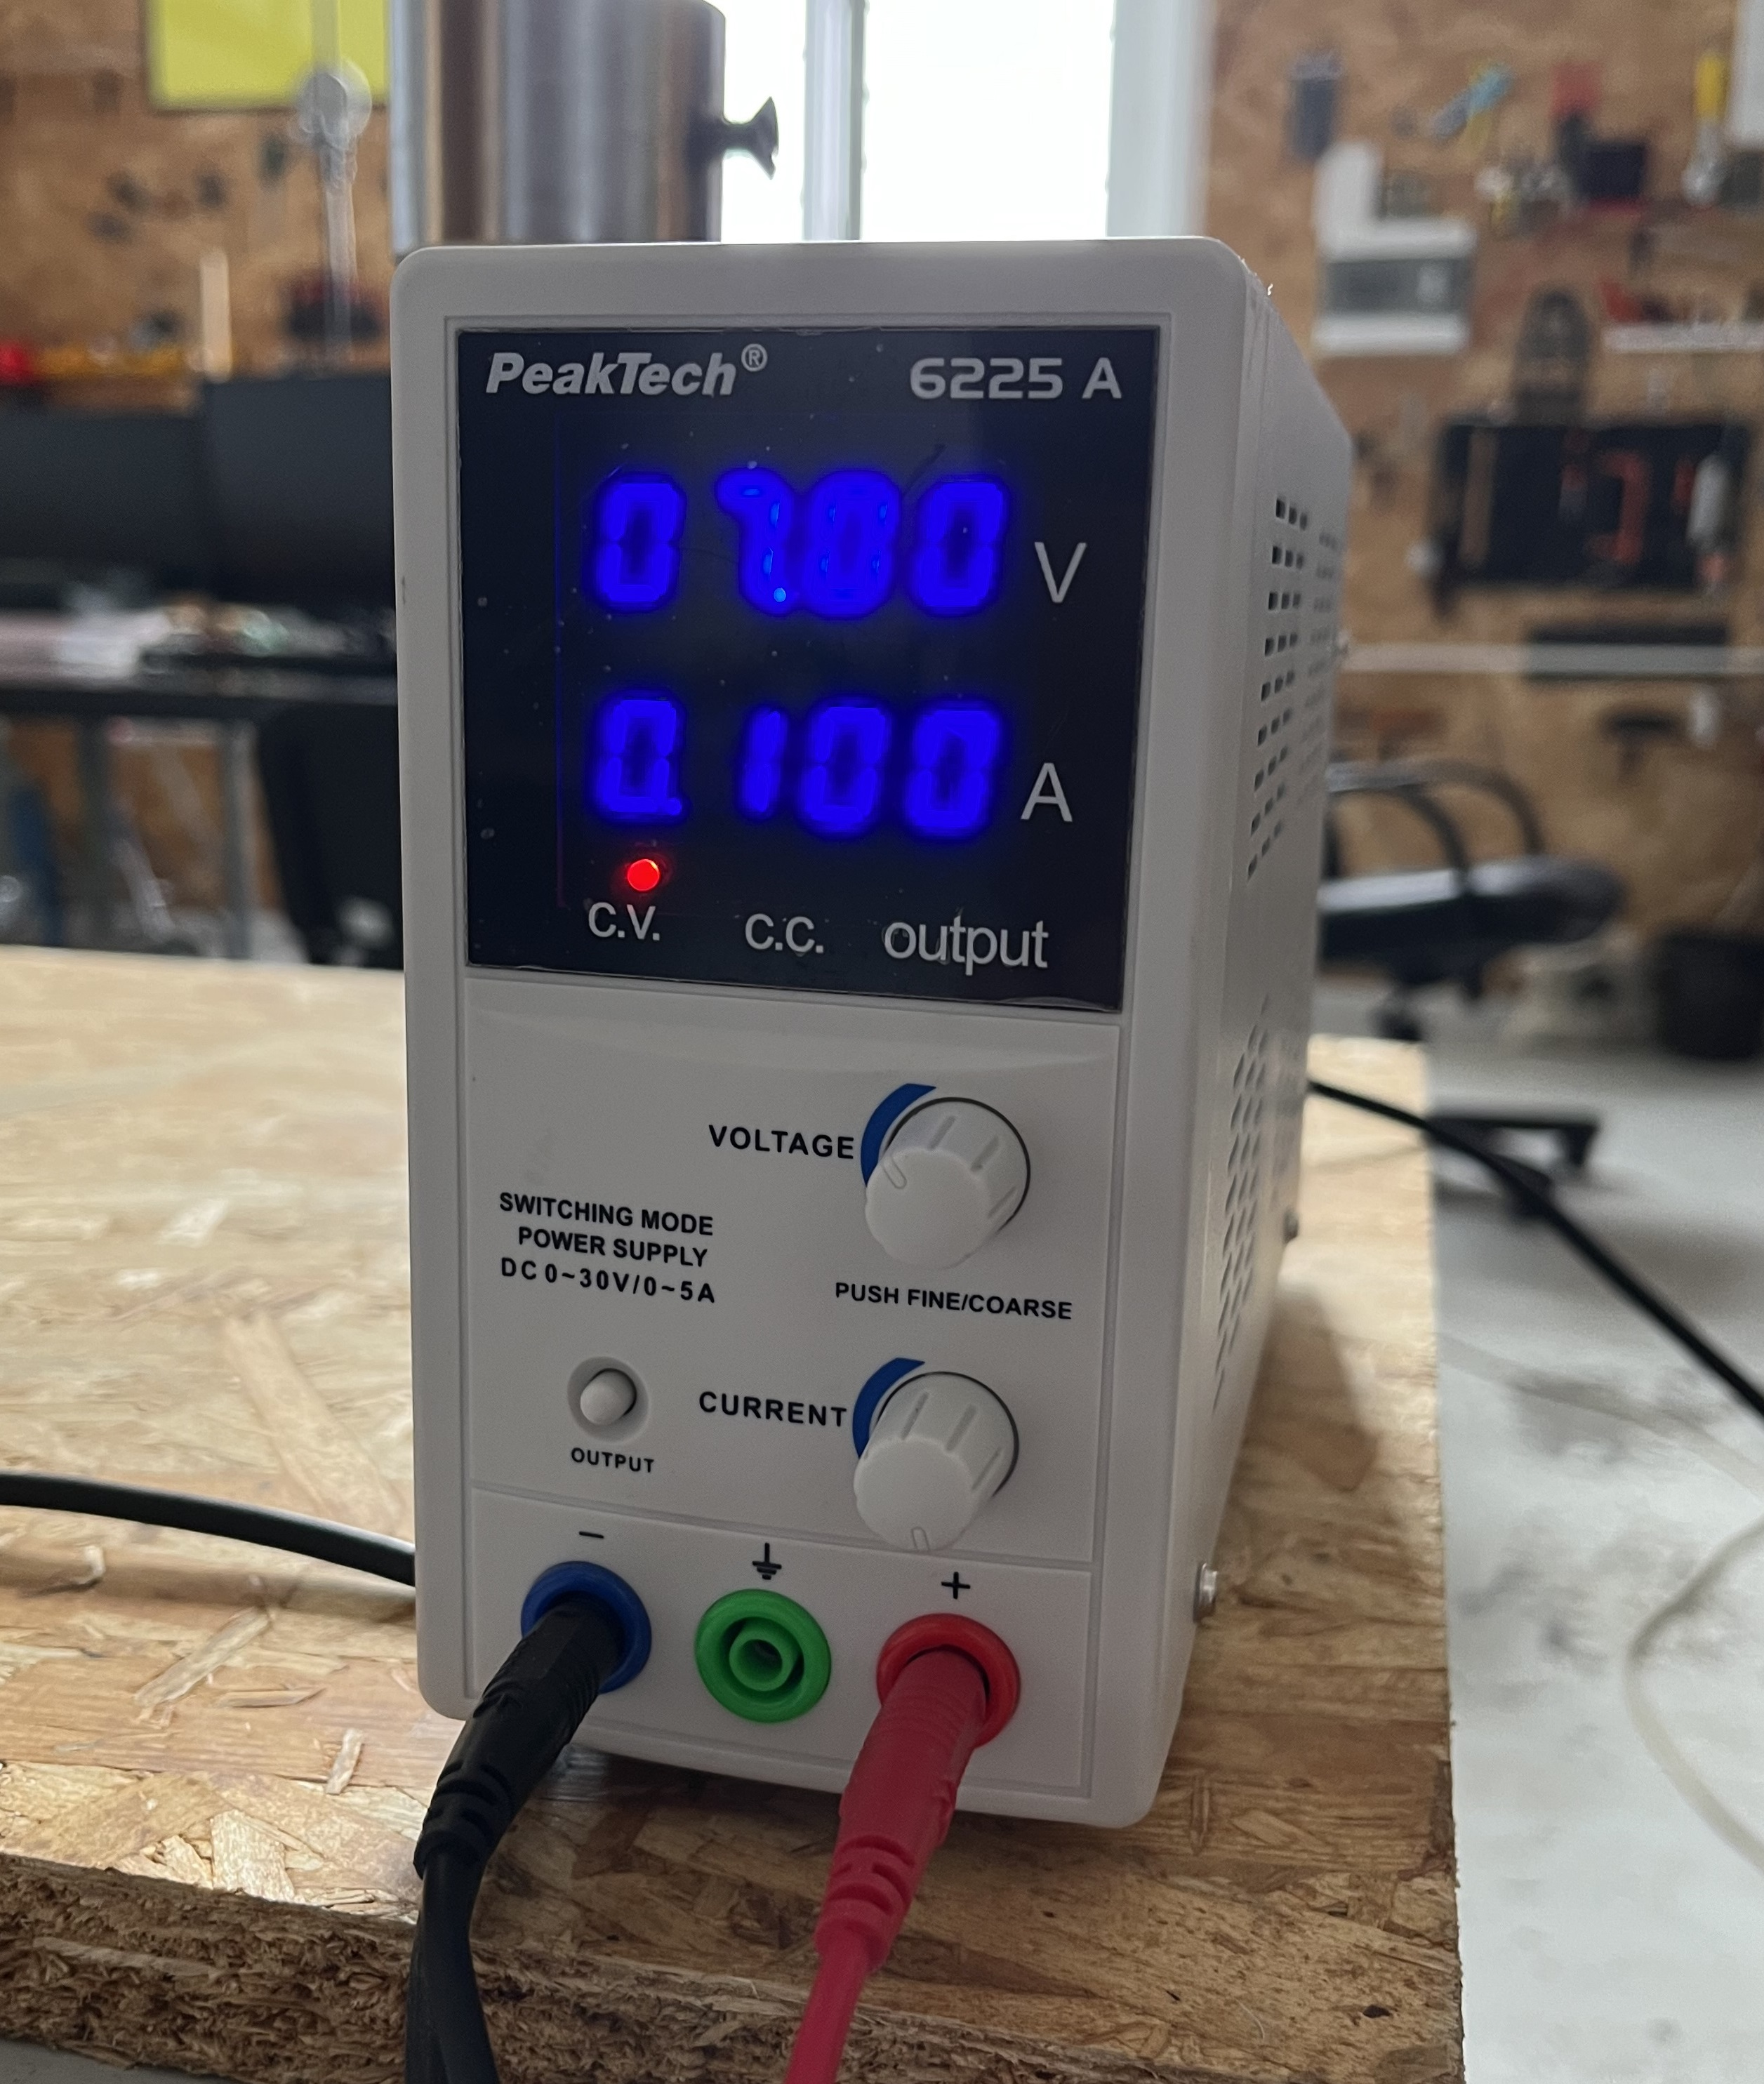
\includegraphics[angle=0,width=0.6\textwidth]{real/peaktech2.jpeg}
    \caption{Eksterno napajanja PeakTech 6225A.}
    \label{napajanje}
\end{figure}

\noindent
Izlazni napon eksternog napajanja PeakTech 6225A se može podešavati od 0V do 30V u koracima od 1V, a izlazna struja od 0A do 5A u koracima od 100mA. PeakTech 6225A koristi mrežno napajanje od 200V do 240V naiymeničnog napona sa učestanošću od 50Hz ili 60Hz.
Prednosti ovog napajanja su mogućnost pružanja velike izlazne snage, dok su mane dimenzije kao i potreba za mrežnim naponom.


\subsubsection{Portabilno eksterno napajanje}

Pošto je napajanje korišćeno za proizvodnju 7V jednosmernog napona i zanemarljivo malu struju od 9mA, moguće je preći na upotrebu baterija od 9V jednosmernog napona. Prednost baterija u odnosu na PeakTech 6225A je portabilnost i to što bateriji ne treba mrežni napon za napajanje. Mana baterije je to što se troši, i nakon nekog vremena će napon pasti ispod minimalnog potrebnog napona za napajanje enkodera i bateriju je potrebno zameniti. Kako bi se produžila upotreba baterije moguće je koristiti dve baterije od 9V jednosmernog napona. Redna veza dve baterije od 9V jednosmernog napona obezbeđuje jednosmerni napon od 18V i ceo sistem može raditi ispravno sve dok napon ne padne ispod 7V jednosmernog napona na baterijama. Ovo dodavanje baterije može produžiti korišćenje baterija značajno duže. Na slici \ref{baterija}. je prikazana korišćena baterija za napajanje, dok je na slici \ref{konektor}. prikazan korišćen konektor za bateriju.

\begin{center}
\begin{minipage}{0.5\textwidth}
\centering
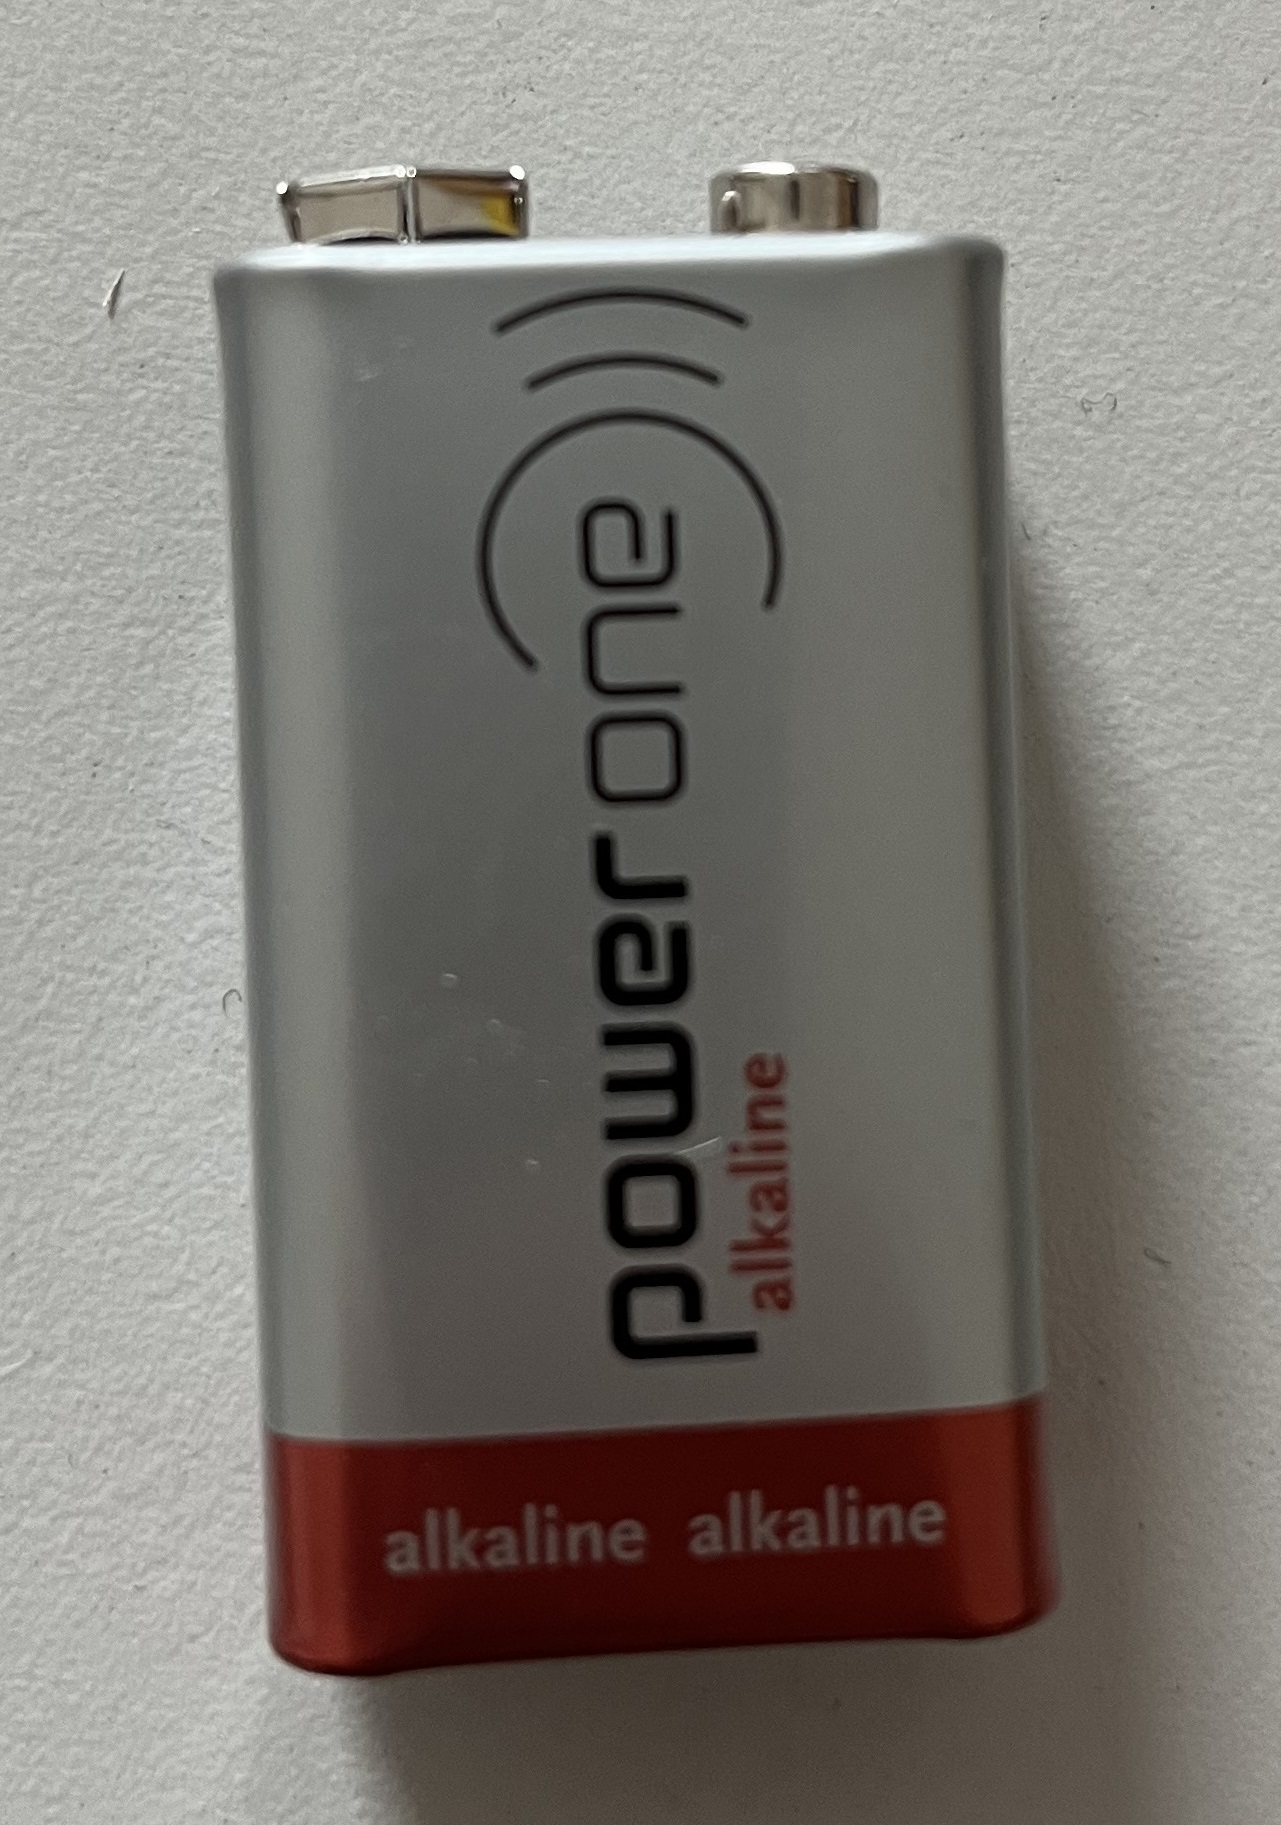
\includegraphics[width=0.7\textwidth]{real/baterija2.jpeg}
\captionof{figure}{Baterija za napajanje.}
\label{baterija}
\end{minipage}%\hfill
\begin{minipage}{0.5\textwidth}
\centering
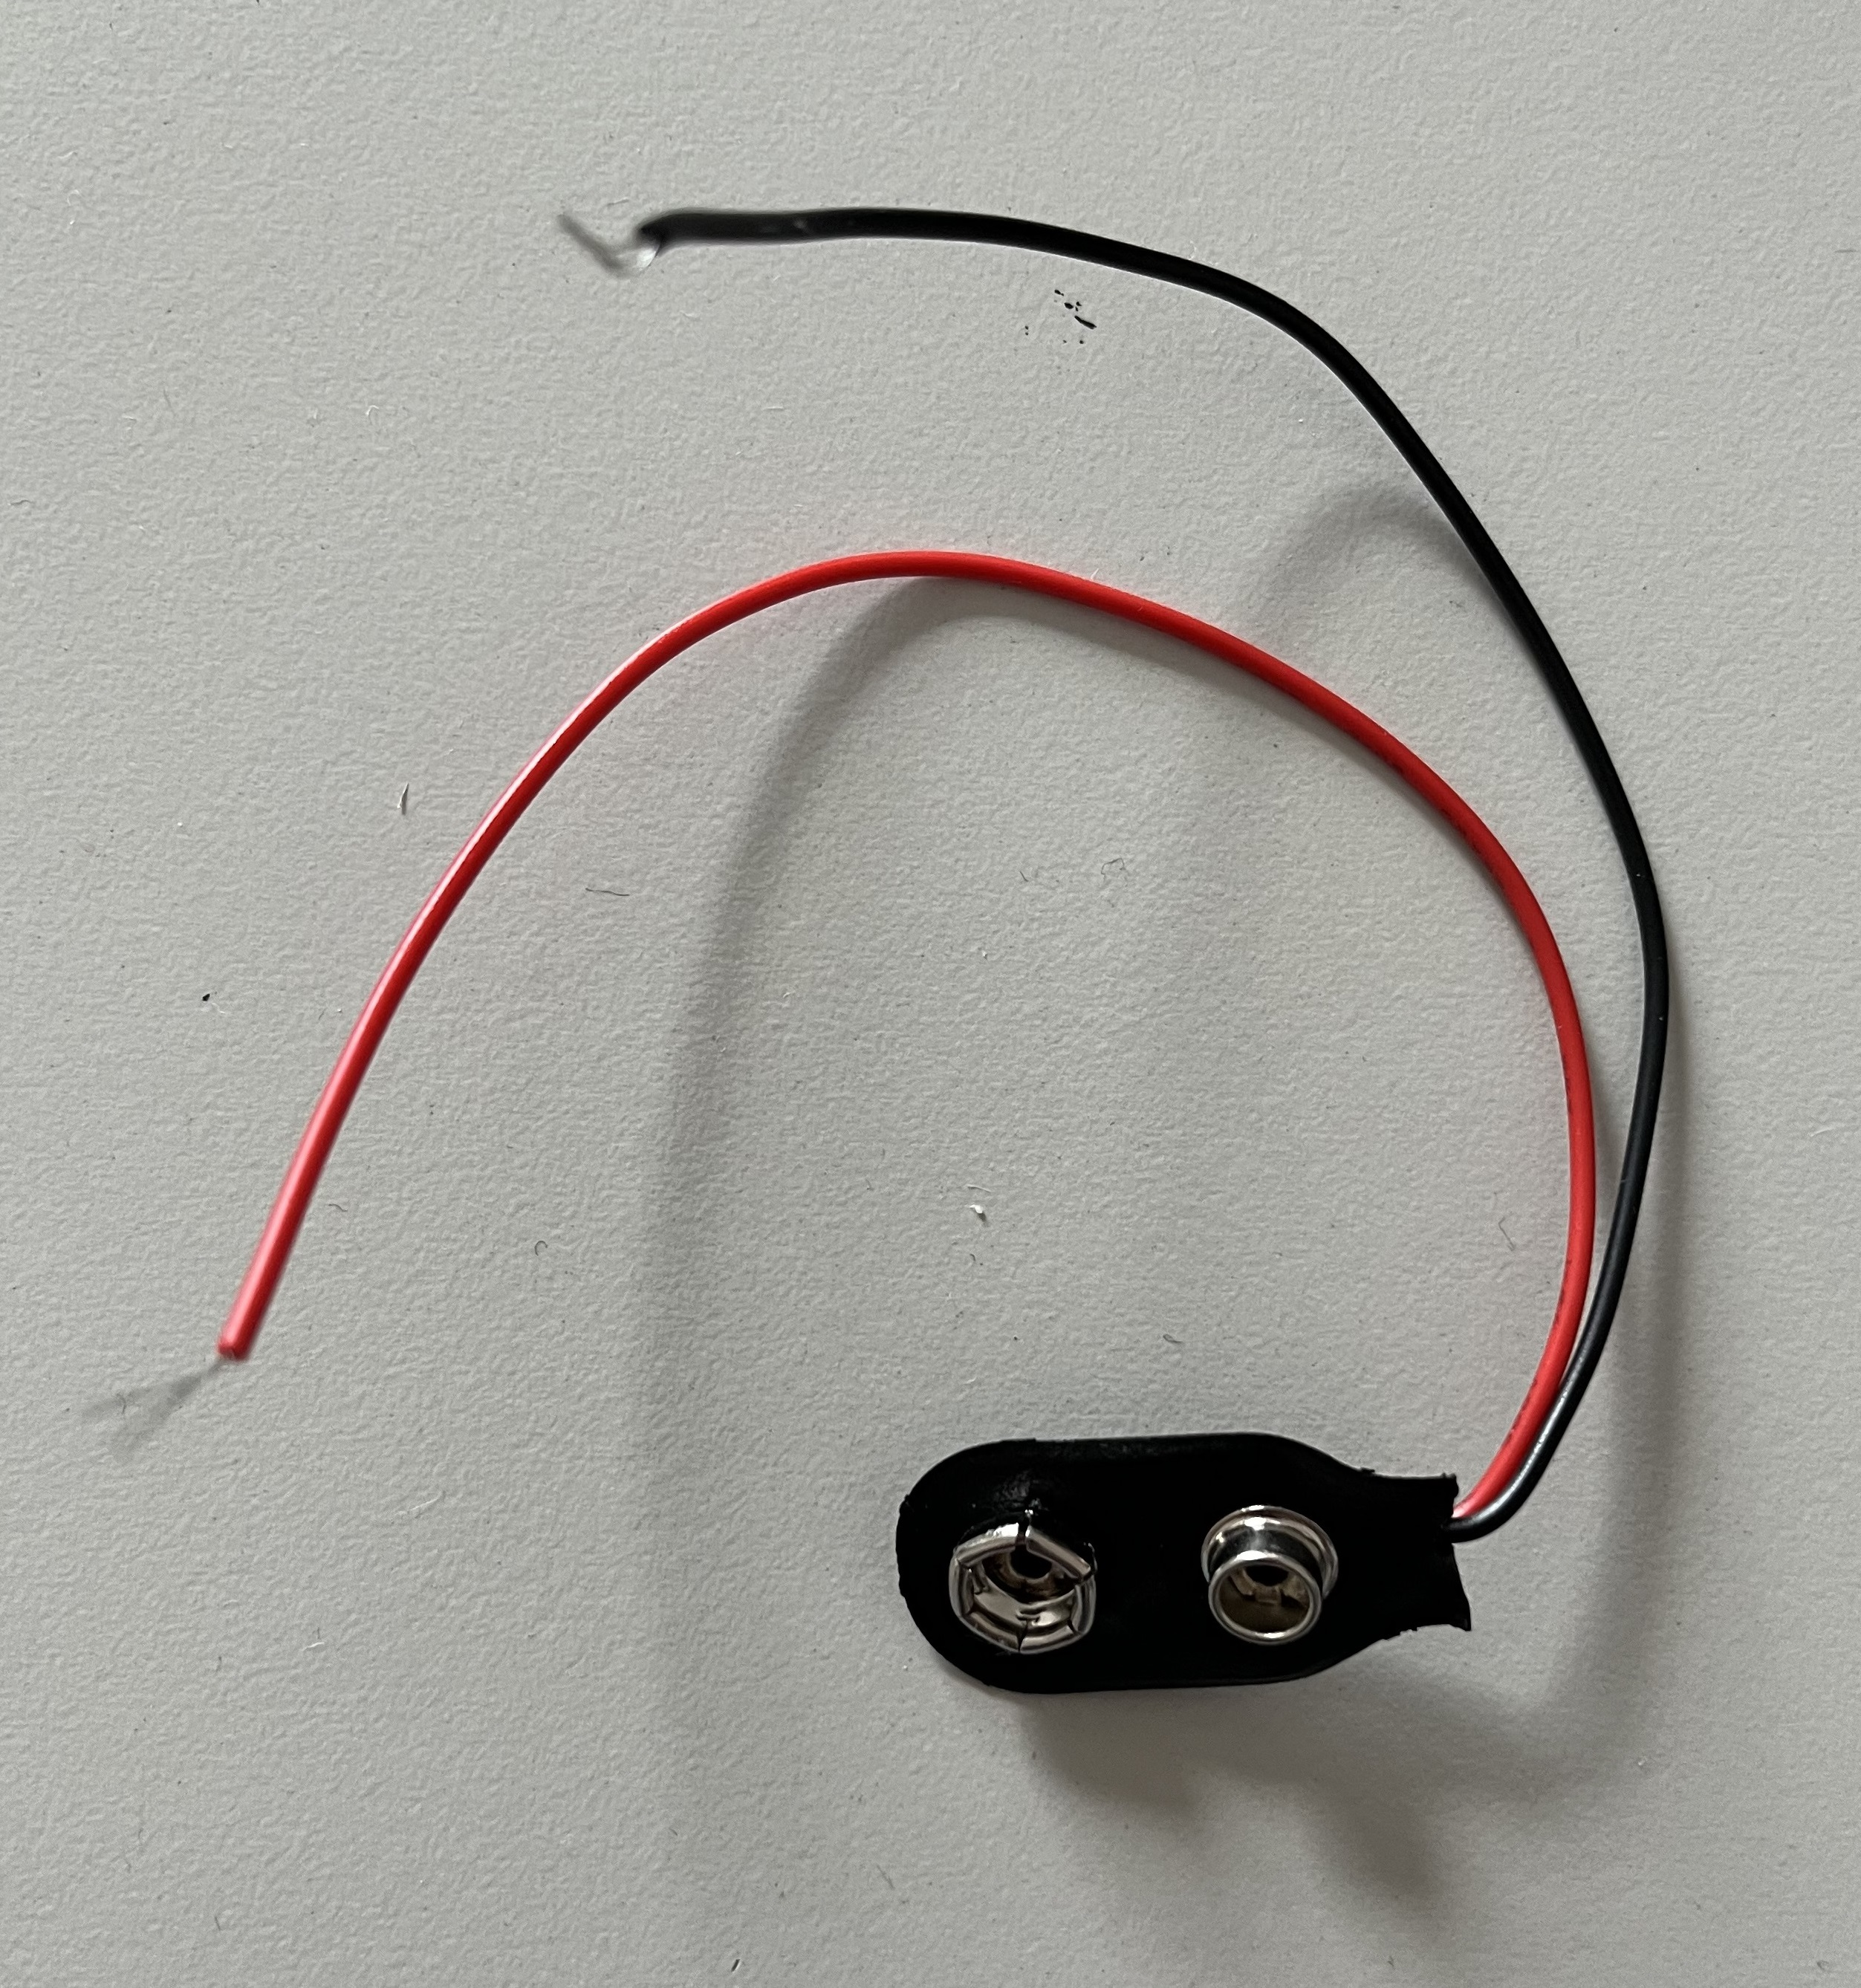
\includegraphics[width=0.9\textwidth]{real/konektor3.jpeg} 
\captionof{figure}{Konektor baterije.}  
\label{konektor} 
\end{minipage}
\end{center}



\subsection{Karakteristike Arduina}

U ovom radu je korišćena Arduino Mega 2560 razvojna ploča za prenos signala sa enkodera na računar. Arduino Mega 2560 je razvojna ploča razvijena od strane Arduino kompanije. Ovaj model se ističe većim brojem digitalnih i analognih ulaza/izlaza, više memorije i većim brojem GPIO pinova u odnosu na osnovni Arduino Uno model. Arduino Mega 2560 koristi ATmega2560 mikrokontroler sa 8-bitnom arhitekturom, koji radi na 16MHz. Poseduje 54 digitalnih ulaza/izlaza (od kojih 15 PWM izlaza) i 16 analognih ulaza. Arduino Mega 2560 ima 256KB fleš memorije za skladištenje koda, 8KB SRAM memorije za promenljive i podatke, i 4KB EEPROM memorije za trajno skladištenje podataka. Komunikacioni interfejsi koje podržava su UART, SPI, I2C za povezivanje sa drugim uređajima kao što su senzori, displeji, moduli za bežičnu komunikaciju itd., dok za komunikaciju sa računarom koristi USB interfejs. Napajanje je takođe preko USB porta, a može biti i eksterno ili preko DC konektora, radni napon je 5V. Arduino Mega 2560 je kompatibilan sa Arduino razvojnim okruženjem (IDE) što omogućava jednostavno pisanje, kompajliranje i postavljanje koda na uređaj. Takođe, kompatibilan je i sa Matlab okruženjem što omogućava lakše programiranje vizuelnih prikaza rezultata. Način na koji je povezan Arduino je preko USB porta na računar, a s druge strane, izlazi enkodera su priključeni na PWM ulaze Arduina kako bi se tumačili kao prekidi i na taj način mođe da se dobije informacija o poziciji klatna. Korišćeni Arduino je prikazan na slici \ref{mega2560}.


\begin{figure}[h!]
    \centering
    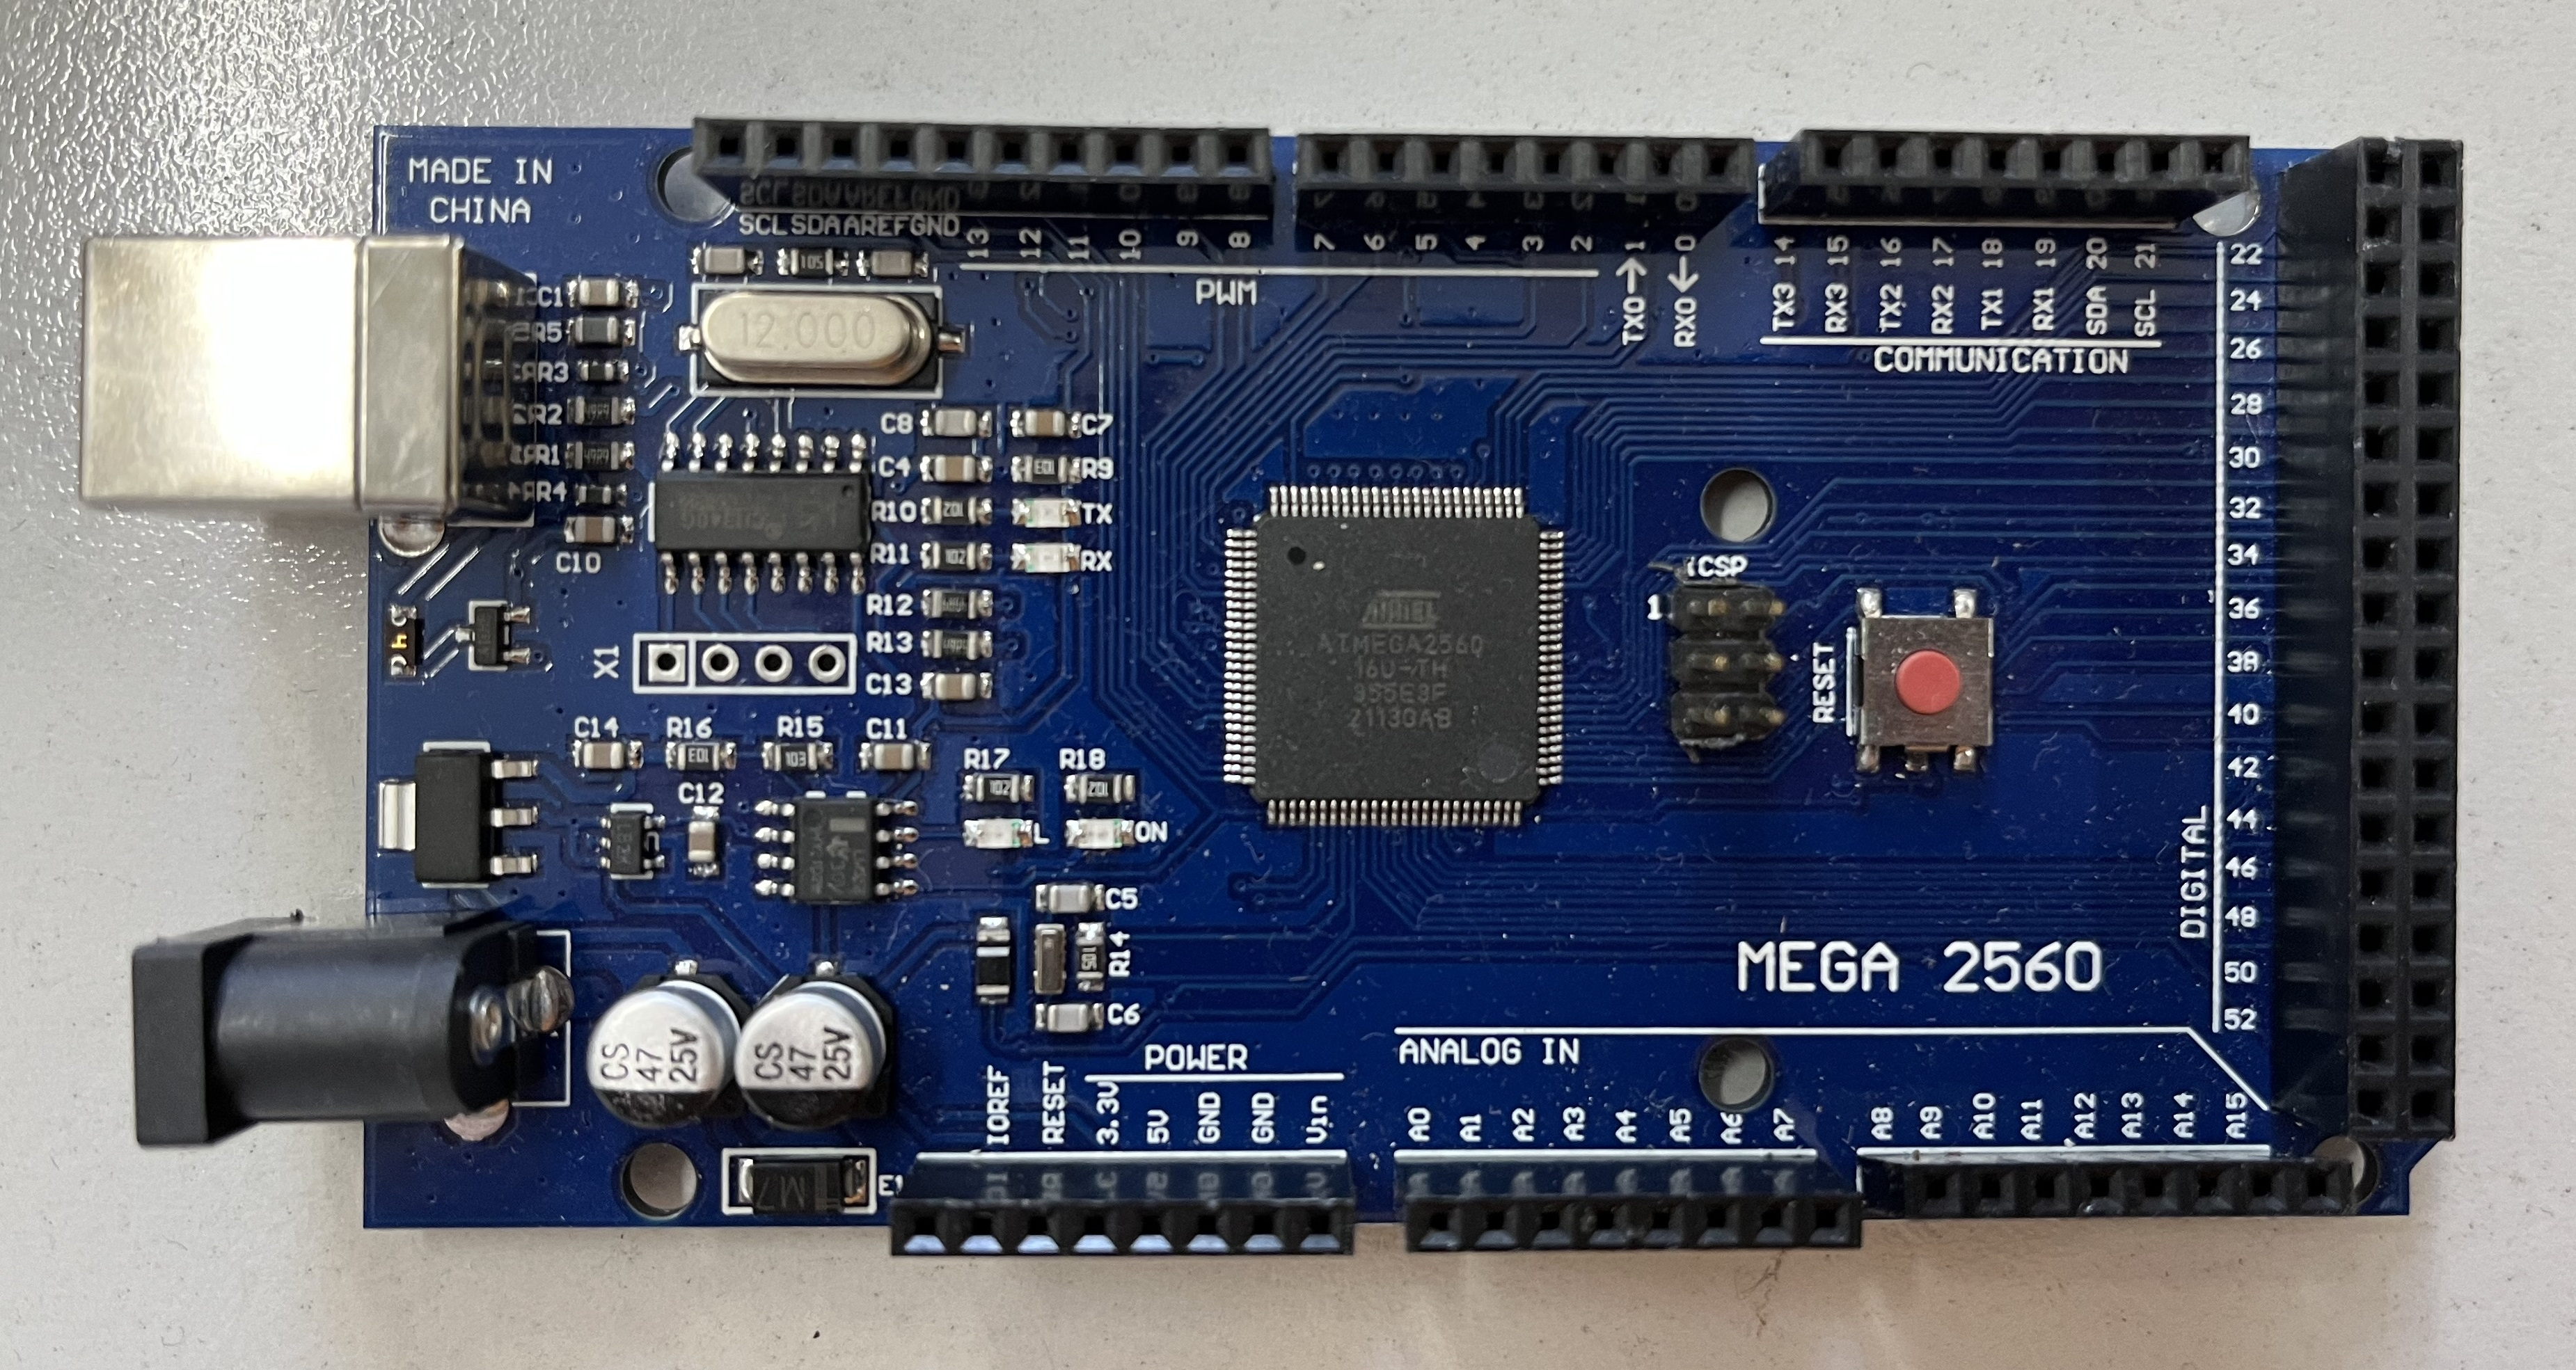
\includegraphics[width=0.8\textwidth]{imgs_real/mega2560_2.jpeg}
    \caption{Arduino Mega 2560.}
    \label{mega2560}
\end{figure}

\noindent
Za precizniju akviziciju su iskorišćeni pinovi za prekide (\textit{interrupt}) 2,3,18,19 na kojima su dovedeni signali A i B sa oba enkodera. U Arduino IDE softverskom okruženju je onda napisan kod koji broji prekide i uzima u obzir u kom smeru se kreće klatno. Uz pomoć ta dva podatka moguće je konvertovati kretanje klatna u cele brojeve koji su direktno povezani sa uglom pod kojim se klatno nalazi. Naime, ako se klatno udaljava od ravnotežnog položaja, broj prekida se povećava, dok se čitanje odvija u toku tog kretanja i može se videti inkrementiranje signala koji predstavlja skaliran ugao. U slučaju suprotnog kretanja koristi se smer kretanja sa enkodera i dodaje se predznak minus na rezultat, ali je suštinski čitanje i tumačenje pozicije identična za oba slučaja. Ovo je jedan od načina implementacije akvizicije signala rotacionog enkodera uz pomoć Arduino Mega 2560 hardvera.
\cite{arduino}\cite{oe}\cite{coolTerm}

Cilj ovog poglavlja je da detaljnije opiše karakteristike korišćenih komponenti u eksperimentalnoj postaci.

\newpage

\section{Rezultati i diskusija}
\label{s:Rezultati}

U ovom poglavlju će biti reči o postavkama, rezultatima i diskusiji dobijenih rezultata i uticaja izmena postavki eksperimenta. 

\subsection{Inicijalna postavka}

U inicijalnoj postavci je korišćen Arduino UNO koji nije imao mogućnosti akvizicije signala sa oba enkodera istovremeno, a i podaci dobijeni tom akvizicijom su morali biti obrađivani u nekom od softverskih alata kako bi se dobio grafik koji je čitljiv. Dodatno, u inicijalnoj postavci nije korišćen prenosni odnos, tako da su dobijeni rezultati bili skoro pa nečitljivi, i nakon toga je odlučeno da se iskoristi Arduino Mega 2560 koji ima mnogo više mogućnosti i bolje opcije za akviziciju signala, kao i dodavanje prenosa kako bi se povećala preciznost. Grafik dobijenih rezultata inicijalne postavke je prikazan na slici \ref{rez0}. radi pokazivanja uticaja izbora odgovarajućeg, odnosno neodgovarajućeg hardvera za akviziciju signala.

\begin{figure}[h!]
    \centering
    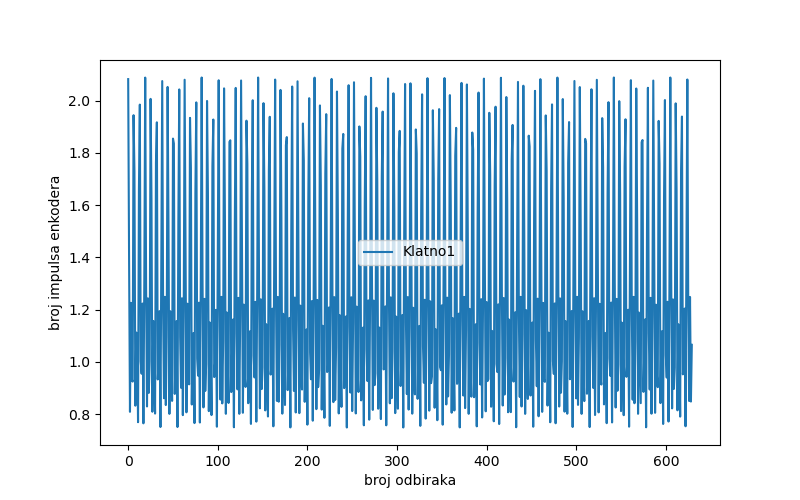
\includegraphics[width=0.95\textwidth]{py_rez/klatno_0.png}
    \caption{Rezultati merenja oscilacija jednog klatna u inicijalnoj postavci.}
    \label{rez0}
\end{figure}

\noindent
Kao što se može videti uz odabiranje neadekvatnog hardvera za akviziciju signala, rezultati su neupotrebljivi, iako je u oba slučaja korišćen isti enkoder. U narednim postavkama je korišćen Arduino Mega 2560 koji pruža bolje mogućnosti za akviziciju signala.


\subsection{Prva postavka}

Uz pomoć jednačina (\ref{eq:diff1}) i (\ref{eq:diff2}), i Python skripte je dobijeno teorijsko očekivanje oscilacija spregnutih klatana prikazano na slici \ref{sim_kretanja}. Zatim se uz pomoć komponenti pomenutih u odeljku \ref{sec:Karakteristike}, i Python softverskog alata dobio rezultat kretanja dva spregnuta klatna koji je prikazan na slici \ref{rez}. Za preciznost prikazanog grafika su zaduženi savremeni hardver za akviziciju signala kao i napravljeni prenosni odnos koji značajno povećava preciznost.


\begin{figure}[h!]
    \centering
    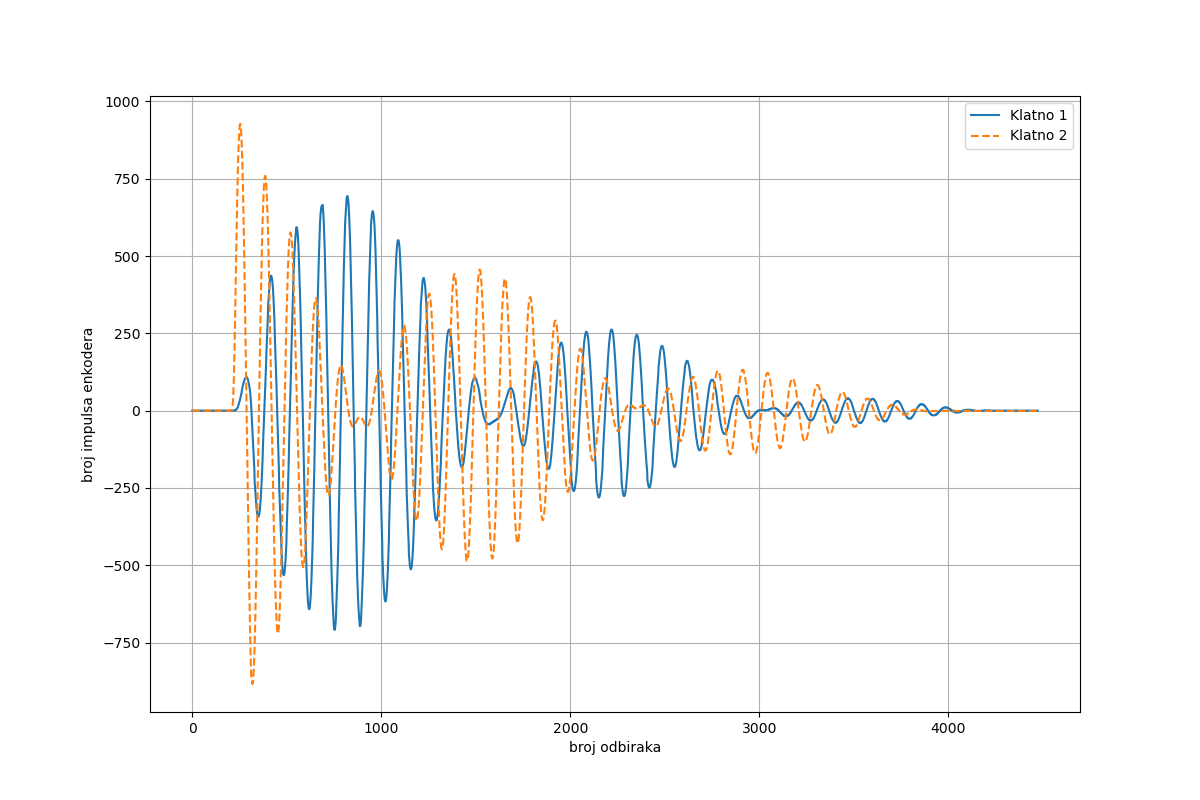
\includegraphics[width=0.95\textwidth]{py_rez/klatno.png}
    \caption{Rezultati merenja oscilacija spregnutih klatna.}
    \label{rez}
\end{figure}

\noindent
Kao što se može jasno primetiti, oblik grafika sa slike \ref{rez} se podudara sa teorijskim očekivanjima, odnosno grafikom dobijenim simulacijom prikazanog na slici \ref{sim_kretanja}. Dodatno, grafici se i razlikuju po brzini opadanja amplitude. Za to su zaduženi otpori koji se javljaju u sistemu, a koji su zanemareni u simulaciji. Otpor u tački vešanja klatna i otpor vazduha imaju najveći doprinos za opadanje amplitude oscilacija. Greška pri merenju je smanjena korišćenjem adekvatnog savremenog hardvera za akviziciju podataka, što smanjuje grešku u oblasti elektronike. Najveći uticaj na neidealnost oscilacija ima sama mehanika i otpori koji se javljaju.


\subsection{Druga postavka}

Prethodni rezultat je imao preveliko prigušenje i nije se moglo dobiti više od nekoliko izbijanja čak i sa velikim početnim uglovima. Pošto su kako je već napomenuto iskorišćeni adekvatan hardver kao i softver za akviziciju podataka, nije bilo moguće dalje unapređivanje po pitanju hardvera i softvera. Jedino što je ostalo je unapređenje mehaničke prirode. Dodati su bolji ležajevi, prenos je poboljšan, dužina neelastičnih šipki je povećana, i mase tegova su povećane, sve u cilju smanjenja uticaja otpora na rezultat. Rezultat dobijen nakon mehaničkih poboljšanja je prikazan na slici \ref{rez2}.

\begin{figure}[h!]
    \centering
    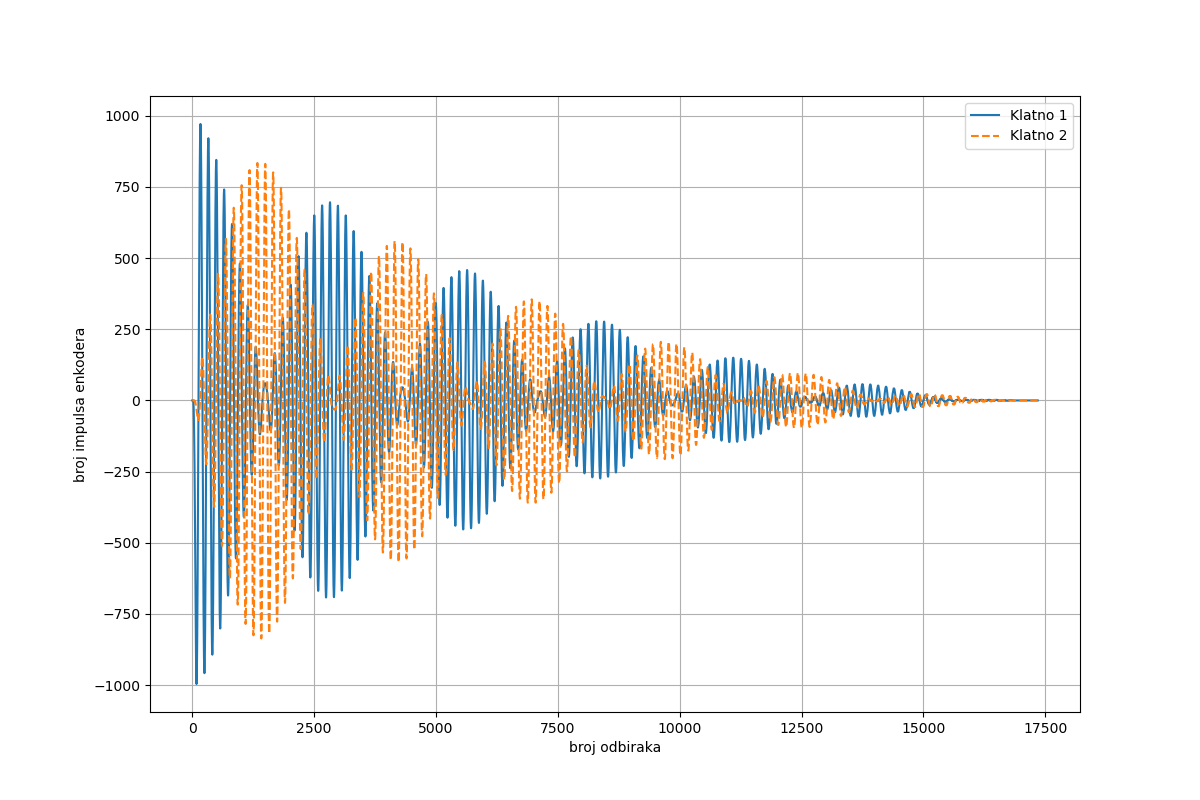
\includegraphics[width=0.95\textwidth]{py_rez/klatno_2.png}
    \caption{Rezultati merenja oscilacija spregnutih klatna.}
    \label{rez2}
\end{figure}



\noindent
Nakon dobijenog željenog rezultata, odrađena su još dva eksperimenta za dobijanje rezultata normalnih modova.


\subsubsection{Mod simetrije}

Za mod simetrije su oba klatna izvedena iz ravnotežnog položaja za približno isti ugao i puštena da osciluju. Način njihovog oscilovanja je prikazan na slici \ref{rez3}.


\begin{figure}[h!]
    \centering
    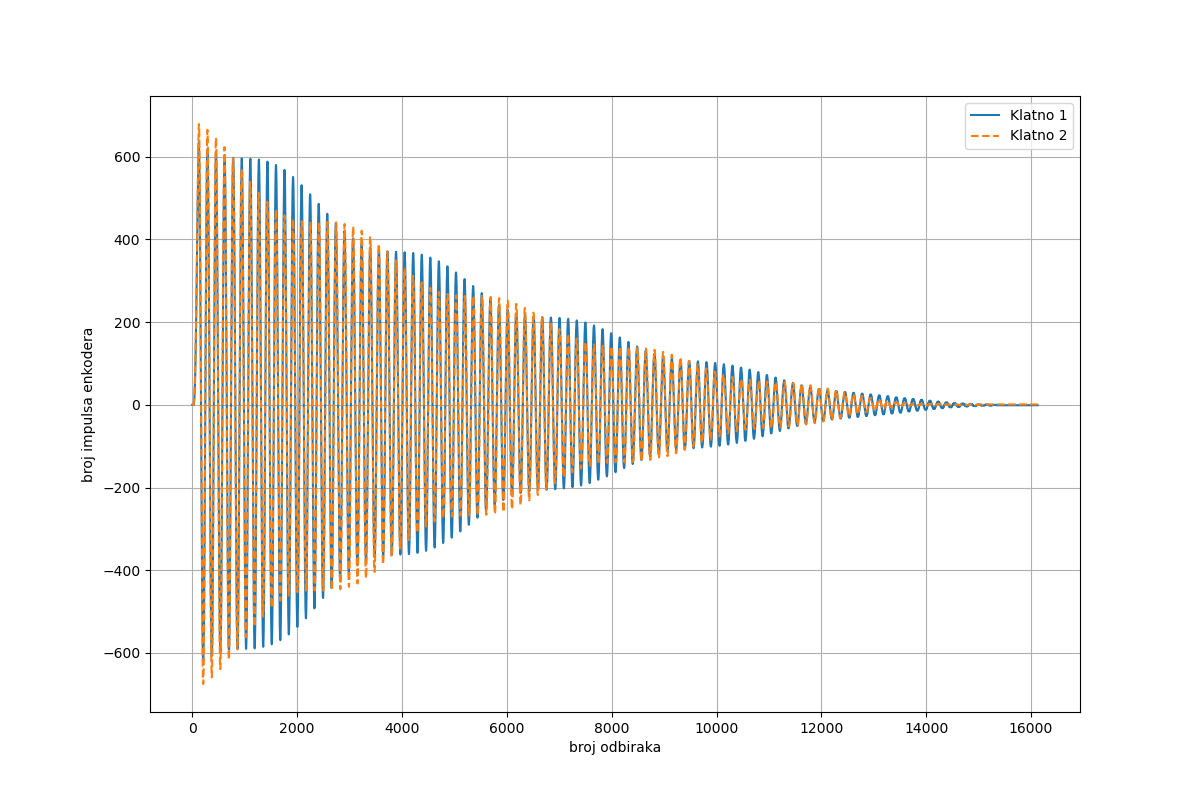
\includegraphics[width=0.95\textwidth]{py_rez/klatno_sim.png}
    \caption{Rezultati merenja oscilacija spregnutih klatna - normalni mod simetrije.}
    \label{rez3}
\end{figure}


\noindent
Sa grafika na slici \ref{rez3}. se može primetiti da postoji mali prenos energije sa jednog klatna na drugo što je posledica neidealnog pokretanja eksperimenta, odnosno početni uglovi klatana nisu bili identični, i to je posledica nepotpunog preklapanja aplituda. Dodatno, sem neidealnog izjednačavanja početnih uglova klatana, na neidealnos preklapanja utiče i sama eksperimentalna postavka, odnosno neidentičnost u samom sistemu kao što su neidentični ležajevi, šipke, tegovi, kaiševi i ostali delovi sistema. Ali se jasno vidi da su, sem malih oscilacija maksimumima amplitude, kretanja identična.


\subsubsection{Mod antisimetrije}

Za mod antisimetrije su oba klatna izvedena iz ravnotežnog položaja za približno isti ugao, ali različitog znaka, i puštena da osciluju. Način njihovog oscilovanja je prikazan na slici \ref{rez4}.


\begin{figure}[h!]
    \centering
    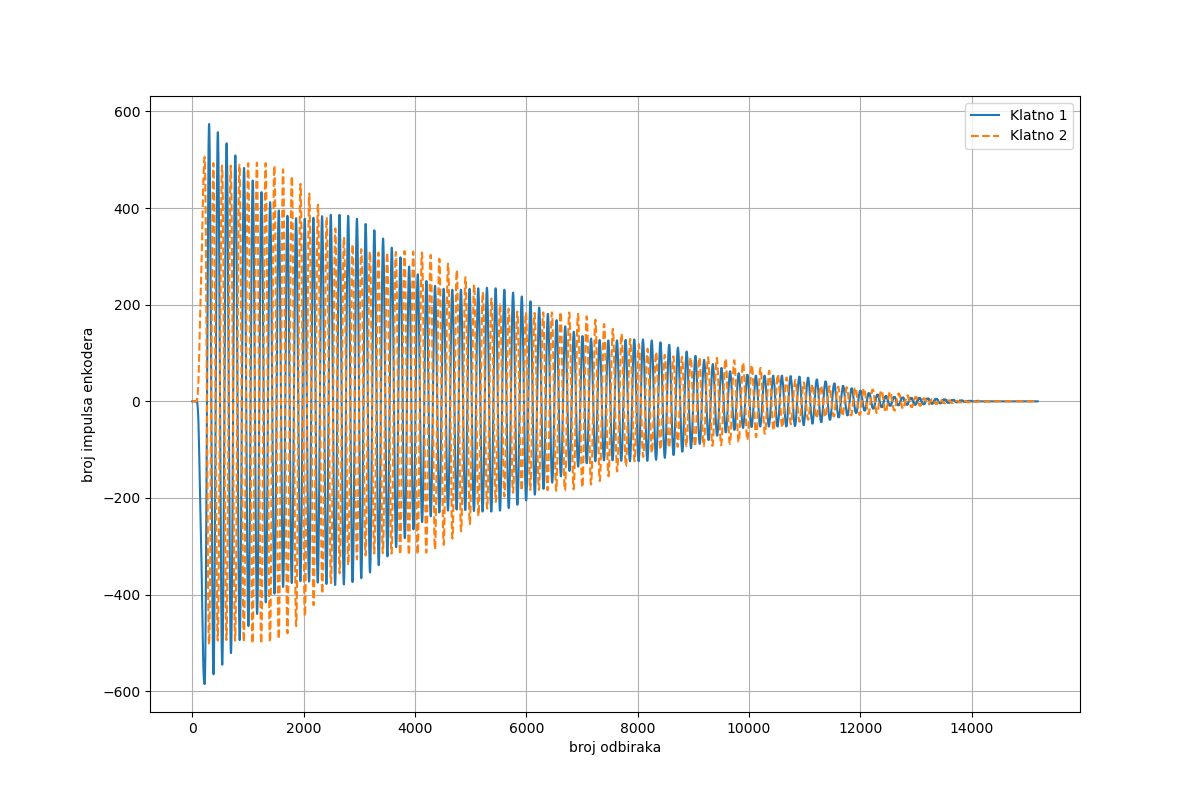
\includegraphics[width=0.95\textwidth]{py_rez/klatno_antisim.png}
    \caption{Rezultati merenja oscilacija spregnutih klatna - normalni mod antisimetrije.}
    \label{rez4}
\end{figure}

Sa grafika na slici \ref{rez4}. se, kao i na prethodnom primeru, može primetiti da postoji mali prenos energije sa jednog klatna na drugo što je posledica neidealnog pokretanja eksperimenta, odnosno početni uglovi klatana nisu bili identični po apsolutnoj vrednosti, i to je posledica nepotpunog preklapanja amplituda. Dodatno, sem neidealnog izjednačavanja apsolutne vrednosti početnih uglova klatana, na neidealnost preklapanja utiče i sama eksperimentalna postavka, što je detaljnije objašnjeno u prethodnom primeru.




Iz ovog primera se može primetiti da jedan isti eksperiment može davati različite rezultate u zavisnosti od izbora hardvera i načina projektovanja sistema. Zato je pre postavljanja eksperimentalne postavke bitno prvo teorijski proceniti rezultate koji su očekivani uz adekvatne aproksimacije kako bi eksperimentalno merenje bilo što preciznije. Zbog aproksimacija u teorijskom očekivanju, odnosno otpora koji se javljaju u realnom eksperimentu postoji greška od teorijski očekivanog rezultata i dobijenog izmerenog rezultata, ali je oblik signala, i način oscilacija isti, što je i bilo potrebno pokazati. Mala odstupanja od teorijskih očekivanja nisu krucijalna sve dok su u granicama zanemarljivih vrednosti i dok se priroda oscilacija dobijena merenjem podudara sa teorijskim očekivanjima.
\cite{dos}


\break


\section{Zaključak}

U ovom radu je izložen postupak projektovanja eksperimentalne postavke spregnutih klatana radi akvizicije signala, i mogući prikaz i obrada podataka dobijenih akvizicijom. Ideja je bila da se uz pomoć rotacionog enkodera i Arduina odradi precizna akvizicija signala koji će se proslediti računaru na dalju softversku obradu i prikaz. Eksperimentalna postavka je sačinjena od spregnutih klatana, rotacionog enkodera, Arduina, napajanja i računara sa odgovarajućim softverom. Dobijanje boljih rezultata je postignuta modifikacijama sistema, prvenstveno korišćenjem adekvatnog savremenog hardvera za akviziciju signala kao i dodavanje adekvatnog prenosa radi povećanja preciznosti pri merenju. Odrađena su sva potrebna merenja i ustanovljeno je da sistem daje teorijski očekivane rezultate što je i pokazano u delu \ref{s:Rezultati}, na slici \ref{rez2}.

Moguće poboljšanje ovog rada je zamena prenosnog mehanizma sa osovinama i stavljanje kliznih ležajeva koji bi pružili još manji otpor i samim tim omogućili duže oscilacije sa manjim prigušenjem. Ideje za dalji rad na projektu je dodavanje jednosmernog motora na osovini koji bi uz korišćenje Arduina i ispisivanje adekvatnog softvera mogao da inicijalno pokretanje oscilacija spregnutih klatana automatizuje tako da čovek nema dodirnih tačaka sa eksperimentalnom postavkom koja bi mogla da bude apsolutno izolovana. Takođe, uz dodavanje prenosa na motor i osovinu, mogao bi se i zadati tačan početni ugao od koga bi oscilacije krenule, za oba klatna. Dodatno, jednosmerni motori bi se mogli koristiti i da vrate klatna u početne položaje odnosno da zaustave oscilacije. U ovom slučaju bi se javio dodatni otpor jer je na osovinu prikačen jednosmerni motor, ali jedna od ideja za rešenje tog problema je dodavanje još jednog jednosmernog motora koji bi služio za povezivanje motora na osovinu, za koje bi takođe bilo potrebno napisati odgovarajući kod u adekvatnom softveru, i u tom slučaju bi cela postavka bila apsolutno automatizovana.

Isprojektovana eksprementalna postavka i upotreba adekvatnog savremenog hardvera za akviziciju signala pokazuje da se teorijska rešenja podudaraju sa dobijenim izmerenim rezultatima. Dodatno, isprojektovani sistem je podložan modifikacijama, kao i upotrebi u drugim eksperimentima uz minimalne izmene.


\break 


\begin{thebibliography}{9}

\bibitem{ems}
Vladimir Rajović, Predavanja iz predmeta Elektronski merni sistemi,
dostupno na \url{http://tnt.etf.rs/~oe4ems/Predavanja.html}, 
poslednji put pristupljeno \today

\bibitem{fiz}
Predrag Marinković, Fizika 1 Skripta,
Beograd, oktobar, 2017.

\bibitem{mit}
Yen-Jie Lee, Predavanja iz predmeta Fizika 3, oscilacije i talasi,
dostupno na \url{https://ocw.mit.edu/courses/8-03sc-physics-iii-vibrations-and-waves-fall-2016/pages/part-i-mechanical-vibrations-and-waves/lecture-1/}, 
poslednji put pristupljeno \today

\bibitem{arduino}
Microchip Arduino Mega 2560, Datasheet,
dostupno na \url{https://content.arduino.cc/assets/ATmega640-1280-1281-2560-2561-Datasheet-DS40002211A.pdf}, 
poslednji put pristupljeno \today

\bibitem{dos}
Vladimir Petrović, Digitalna Obrada Signala,
dostupno na \url{http://tnt.etf.rs/~19e043dos/vezbe.php},
poslednji put pristuljeno \today

\bibitem{oe}
Radivoje Đurić, materijali za predmet Osnovi Elektronike,
dostupno na \url{http://oe2oe.etf.bg.ac.rs/},
poslednji put pristupljeno \today

\bibitem{encArduino}
Članak na temu "\textit{How rotary encoder works and interface it with Arduino}",
dostupno na \url{https://lastminuteengineers.com/rotary-encoder-arduino-tutorial/},
poslednji put pristupljeno \today

\bibitem{coolTerm}
Dokumentacija za softver "\textit{CoolTerm}",
dostupno na \url{https://freeware.the-meiers.org/CoolTerm_ReadMe.txt.html},
poslednji put pristupljeno \today



\end{thebibliography}



\newpage

\begingroup
\let\clearpage\relax
\listoffigures
\endgroup

\end{document}



